\newpage
\phantomsection
\chapter{Experimental applications}\label{chap:results}

In the previous chapter, the SHARP technique was explained in detail, including additional steps and modifications to address specific issues encountered in certain instances, as well as a proof of concept experimental validation using a straightforward to image sample with prominent structures, convenient to readily visualize and verify computational refocusing. Also, the CTNode technique was described and evaluated with a simulated tomogram.  In this chapter, experimental operation of SHARP is demonstrated with samples with medical relevance including \textit{ex vivo} and \textit{in vivo} imaging, to show the potential of SHARP to improve the quality of OCT tomograms in order to provide more detailed information of tissue and to facilitate visualization of images for a improved analysis of specialists, more importantly in intensity-based imaging but in polarization-sensitive imaging as well. Additionally, experimental application of SHARP is complemented with the previously developed technique TNode and the new proposal CTNode, to provide a more significant improvement of image visualization.

First experimental demonstration is presented in anterior segment imaging of an excised swine eye, where SHARP is complemented with TNode and CTNode independently, being this an application with great relevance in OCT given that the anterior segment possesses structures with fundamental roles for vision, including cornea, limbus, iris, sclera, among others. An additional demonstration of performance of CTNode is then presented in human retina \textit{in vivo}, independently of SHARP.  A second demonstration of SHARP is presented in catheter-based imaging, which is the second largest imaging modality in OCT after ophthalmic-OCT, using a dataset from the air-way of a swine acquired \textit{in vivo}. An additional \textit{in vivo} demonstration is showed in skin imaging of human hand dorsal where involuntary sample motion arising from pulse heartbeat and respiration must be corrected. Finally, the operation of SHARP in polarization-sensitive OCT is demonstrated in the limbal region of the excised swine eye, showing computational refocusing of polarimetric parameters.

The experimental data-sets of the anterior segment and human skin were acquired with the bench-top system used for the proof of concept experiment, varying in some cases the scan lens and sampling configuration accordingly. The endoscopic dataset that was provided by NinePoint Medical. The human retina dataset was acquired with a bench-top retinal SSOCT system integrated in a modified commercial ophthalmic interface~\cite{Braaf2018_Complex} . Specific relevant parameters used in each experiment are described in the corresponding section.

\section{Anterior segment imaging \textit{ex vivo}}

The eyeball is in general divided into two main sections for its study; the anterior segment depicted in Figure~\ref{fig:eyeSchematic} and the posterior segment. The former is primary responsible for light collection and image formation by the cornea and the lens, and there are additional functional structures that support the normal operation of the eye including the iris, sclera, and ciliary body. OCT systems  for anterior segment imaging typically have a large depth of field of $\sim$3~mm to provide focused images across the entire axial extent of the anterior segment that is relatively large, but this implies a coarse lateral resolution. In some cases, the local structure of specific tissue is desired, for instance in the study of corneal layers thickness and stroma arrangement~\cite{Huang2015_Anterior}, achievable using high-resolution systems at the cost of having a relatively short depth of field.

\begin{figure}[htb!]
	\centering
	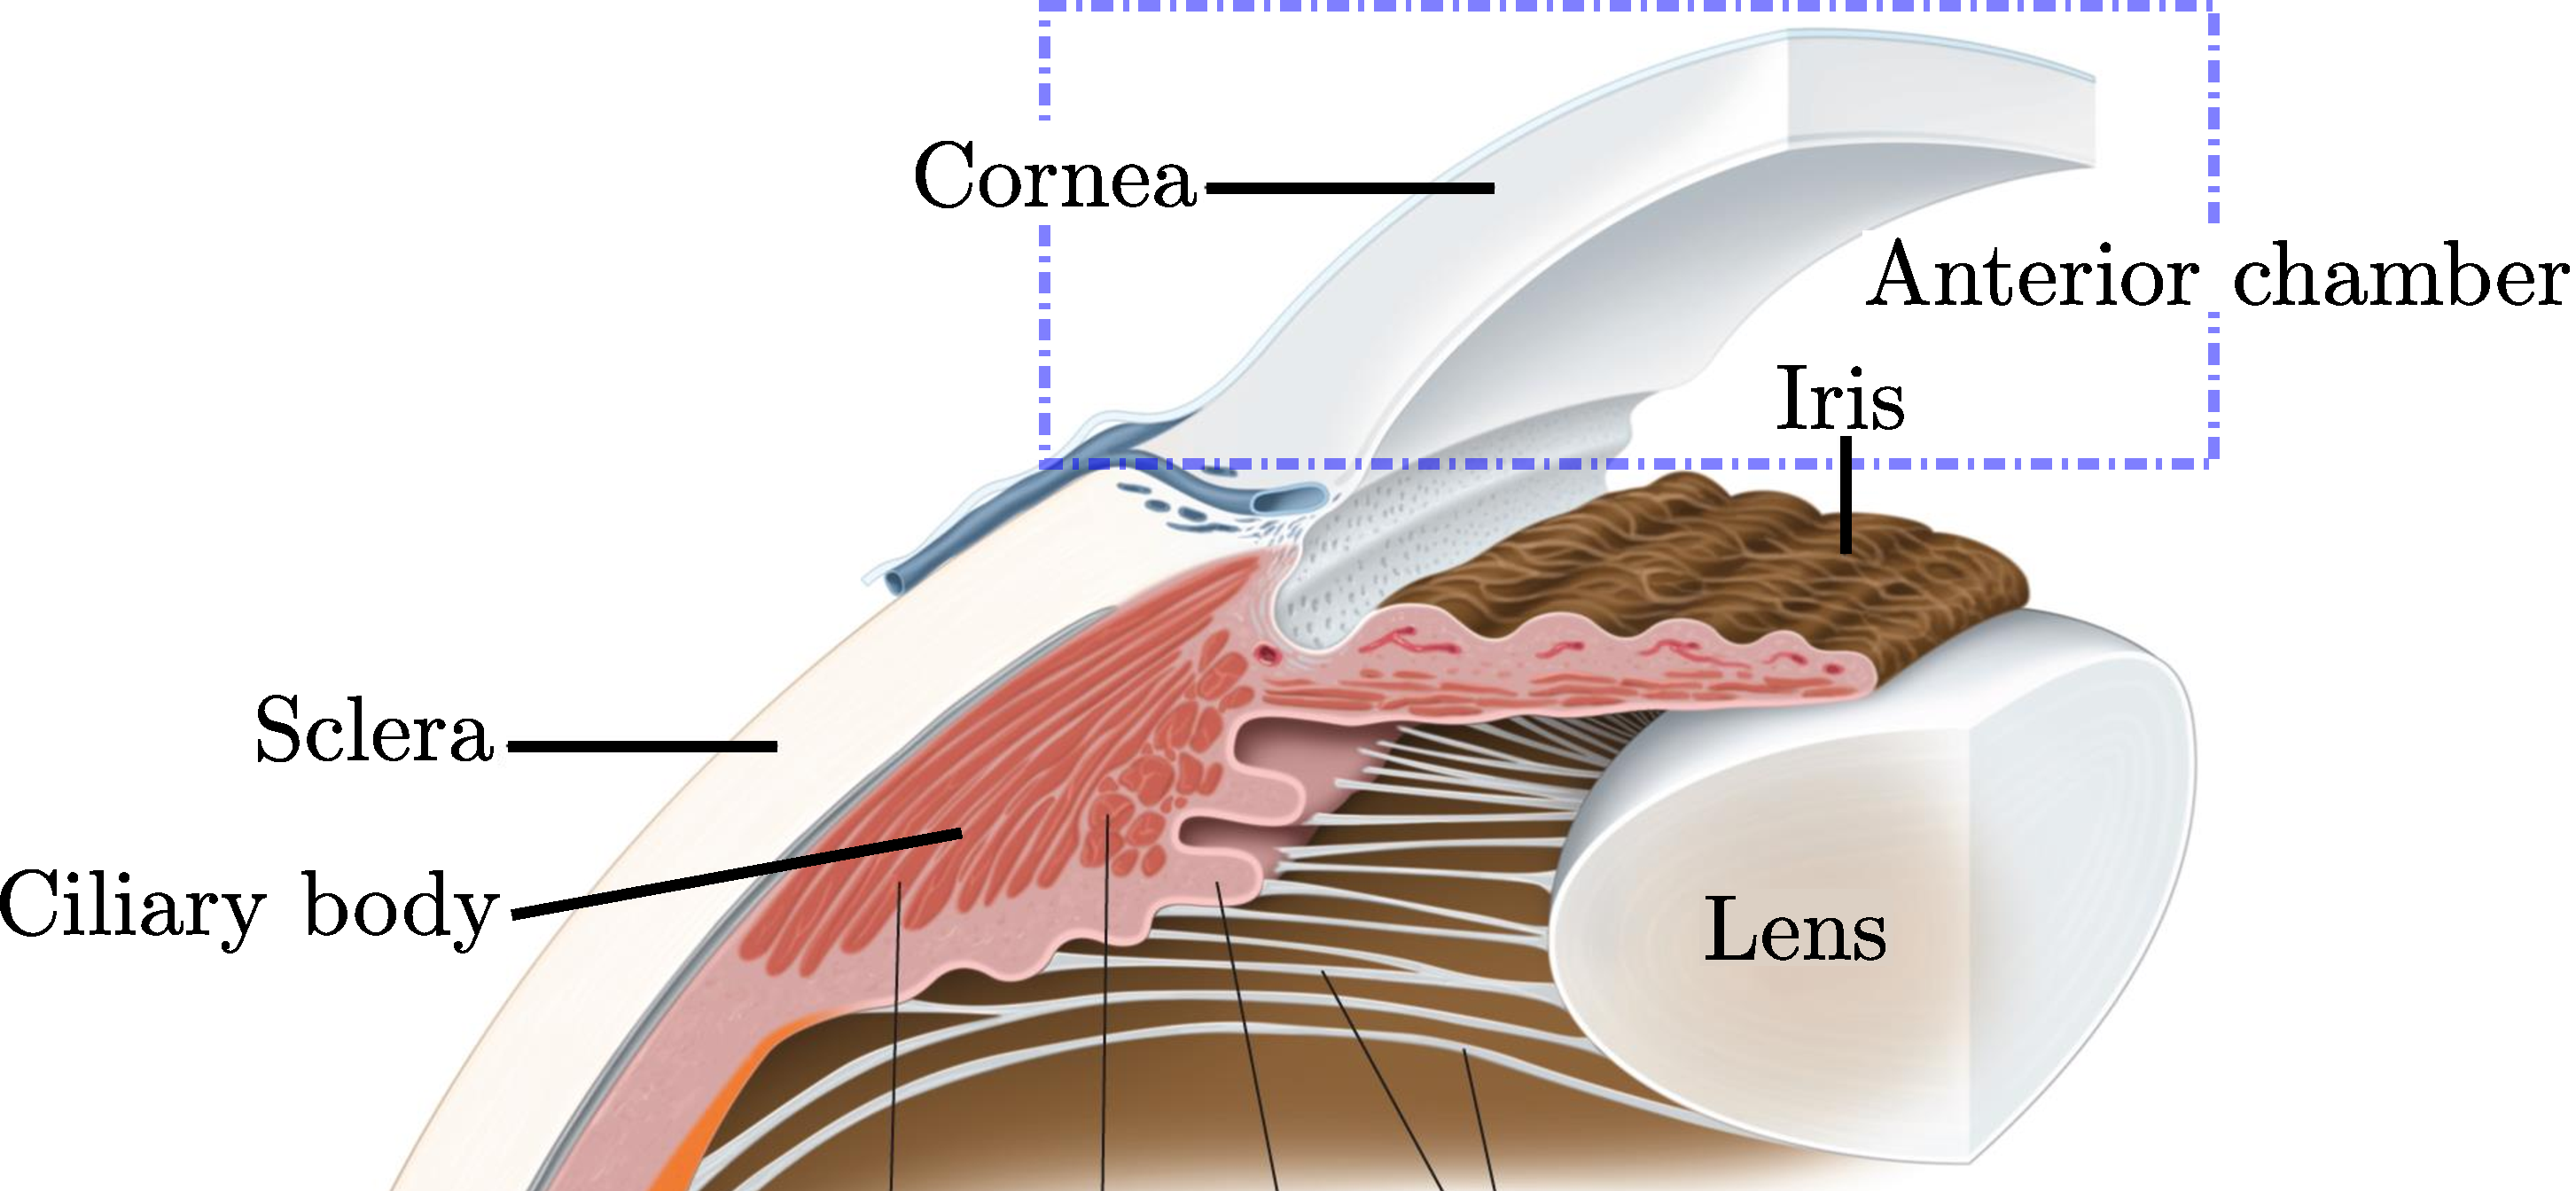
\includegraphics[width=.65\textwidth]{Figures/Results/EyeSchematic.pdf}
	\caption[Illustration of anterior segment anatomy.]{Illustration of anterior segment anatomy. [Adapted from \href{https://www.aao.org/image/anterior-segment-anatomy}{$\copyright$ 2020 American Academy of Ophthalmology}].}
	\label{fig:eyeSchematic}
\end{figure}

Computational refocusing has potential to extend the depth of field in anterior segment imaging in order to provide images with high lateral resolution in an extended depth covering a larger axial range of anterior segment~\cite{Wang2019_Cellular}. As an initial experimental demonstration, the SSOCT system used in the proof of concept experiment previously described was used to image the anterior segment of an excised swine eye, emphasizing in the cornea, around a region similar to that enclosed by blue rectangle in Fig.~\ref{fig:eyeSchematic}. From the measured tomogram, an ROI of 700 samples per A-line, 768 A-lines per B-scan and 256 B-scans was selected, covering a lateral field of view of 6$\times$2~mm$^2$ in an axial ranging of 4~mm in air. Two data-sets were acquired; a reference tomogram with the focal plane located at the paracentral zone of the cornea, and an OoF tomogram with the focal plane located at the iris, not visualized in the selected ROI. Figure.~\ref{fig:ASImaging}(a) shows a B-scan of the original tomogram where defocus is evident in all the corneal layers and structures inside the stroma. Due to the confocal gating, there is a drop in signal-to-noise ratio (SNR) due to the large offset from the focal plane, observed as a low contrast between signal level in corneal tissue and noise floor level in regions having not signal from tissue.

Standard SHARP procedure was applied to the OoF tomogram, using Legendre polynomials $P_2,\ P_3,\ P_4,$ and $P_5$. The correction weights in $y$ were set equal to those found in $x$ given that the optimization procedure in $y$ was prone to fail at certain planes, possibly because there is not enough signal information for a robust estimation of the image quality metric, since the FoV in $y$ is small and the structures are oriented toward the $y$ axis. Fig.~\ref{fig:ASImaging}(b) shows that using the optimum filter [$\tilde{\Omega}(q_x,q_y)$] alone (i.e. setting phase filter $\tilde{\varphi}$ to zero) is very effective at reducing noise in this particular case where SNR in intrinsically low, achieving a floor noise reduction of $\sim$6~dB, which improves overall contrast. However, optimum filter alone does not improve the blur, contrary to Fig.~\ref{fig:ASImaging}(c) that shows that after applying SHARP structures appear both sharper and with better contrast. Image improvement with SHARP can be observed in the fibrilar structure in the stroma, but presence of speckle hinders visualization and assessment as noted when comparing insets in Figs.~\ref{fig:ASImaging}(a)-(c). For this reason, images were despeckled with TNode technique, known to preserve resolution and improve image contrast~\cite{Cuartas-Velez2018_Volumetric}, in order to facilitate visual inspection and assessment, using similarity and search windows of 5$\times$5$\times$5 and 15$\times$1$5\times$15 pixels ($z\times x\times y$) respectively, and filtering parameters $h_0 = 0.035$ and $h_1 = 0.010$. B-scans of the original and SHARP tomograms are shown in Figs.~\ref{fig:ASImaging}(d) and (e) after despeckling with TNode, where successful refocusing is distinguishable in SHARP image, which approaches to the image quality of the despeckled reference B-scan in Fig.~\ref{fig:ASImaging}(f), being loss in signal strength the major difference and a significant drawback in CAC.

\begin{figure}[htb!]
	\centering
	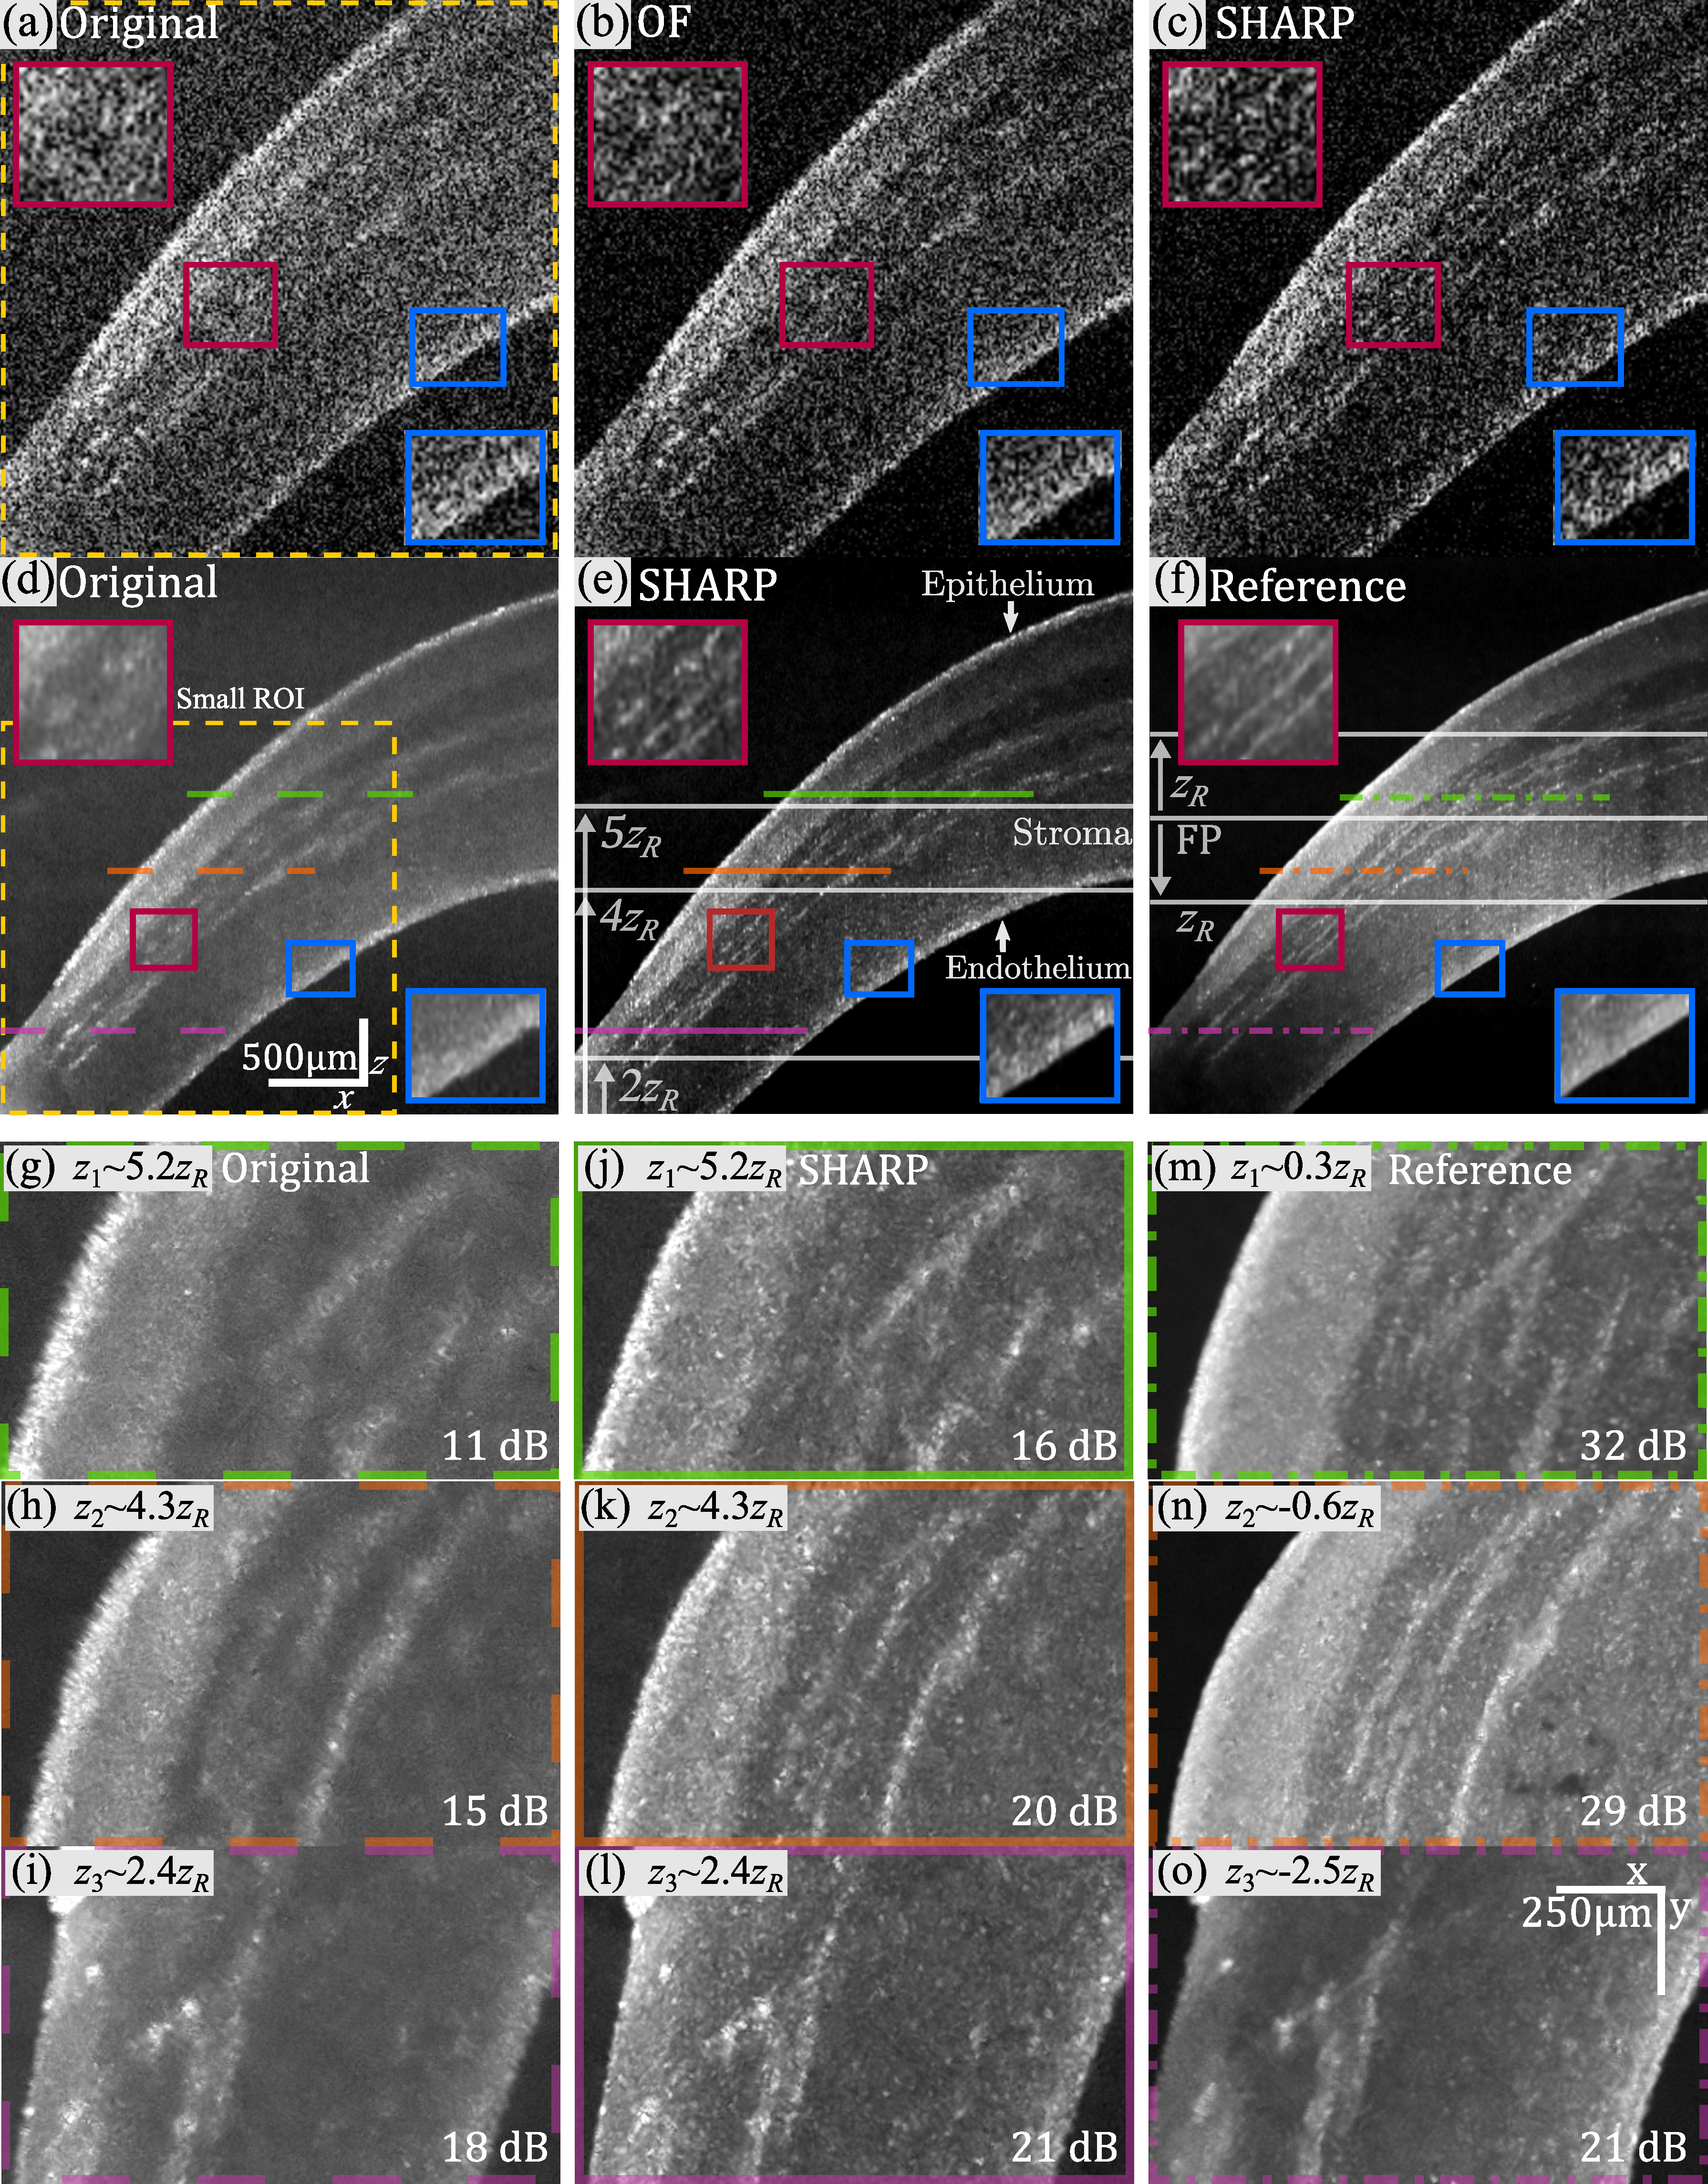
\includegraphics[width=\textwidth]{Figures/Results/ASImaging.pdf}
	\caption[Application of SHARP in anterior segment of excised swine eye.]{Application of SHARP in anterior segment of excised swine eye. Small ROI B-scans: (a) original, (b) OF, and (c) SHARP. Full ROI B-scans after despeckling with TNode: (d) original, (e) SHARP and (f) reference (FP: focal plane, in (a)--(e) FP is in iris, out of image range). \textit{En face} at depths $z_i$ marked with lines in the B-scans: (g)--(i) original, (j)--(l) SHARP and (m)--(o) reference. Each \textit{en face} image shows its dynamic range.}
	\label{fig:ASImaging}
\end{figure}

Figures~\ref{fig:ASImaging}(g)--(o) show three despeckled \textit{en face} views of the original, SHARP and reference tomograms at three depths indicated by lines in Figs.~\ref{fig:ASImaging}(d)--(f). The dynamic range of each \textit{en face} view was adjusted to equalize the contrast for visual comparison. Blurring increases towards the cornea apex in the original views in Figs.~\ref{fig:ASImaging}(g)--(i). In contrast, SHARP views [Figs.~\ref{fig:ASImaging}(j)--(l)] have perceptually very similar resolution at all depths, enabling improved visualization of structures inside the stroma and clearer boundaries of the corneal epithelium, resembling reference images Figs.~\ref{fig:ASImaging}(o)--(m). These results show that SHARP could enable the examination of the iris and the full cornea in a single-shot acquisition with higher lateral resolution than currently possible, facilitating the accurate determination of parameters of clinical interest such as the stromal demarcation line and tissue layer thicknesses with existing OCT systems without regard to phase noise. Finally, the combination of SHARP and TNode provided a significant improvement of image quality compared to the original tomogram, in terms of resolution improvement, noise reduction and contrast.

\subsection{CTNode in combination with SHARP}

Back-scattering of cornea is relatively low because its constitutive tissue is inherently translucent for functional purposes, making that cornea stroma generally exhibits low to medium SNR, even lower in the presence of aberrations. In the previous demonstration of SHARP, the optimum filter shown to be a key tool to improve visualization of results in terms of noise suppression, providing an extended dynamic range. The aim now is to combine CTNode with SHARP to further improve contrast by reducing noise floor level.

After applying SHARP to the tomogram of previous demonstration, CTNode was applied using search and similarity windows of 11$\times$11$\times$11 and 3$\times$3$\times$3, respectively, and $h = 0.15$. Figure~\ref{fig:ASImaging_CTNode} shows a selected B-scan of the original tomogram, after SHARP and after subsequent CTNode. The top value of the dynamic range of all images is the same but the lower limits were equalized to the noise floor level ($\mu_N$) of each image, computed as the average intensity within the blue rectangles in Figs.~\ref{fig:ASImaging_CTNode}(a)-(c), in order to match the visual contrast at the cost of having different dynamic ranges. More specifically, original B-scan in Fig.~\ref{fig:ASImaging_CTNode}(a) has a noise floor level of 56~dB and a dynamic range of $16$~dB, in SHARP B-scan in Fig.~\ref{fig:ASImaging_CTNode}(b) the noise floor was reduced by 6~dB, allowing to incraese dynamic range to 22~dB and after CTNode noise floor was additionally reduced by 5~dB, for a total reduction of 11~dB, allowing to increase dynamic range to 27~dB.

\begin{figure}[htb!]
	\centering
	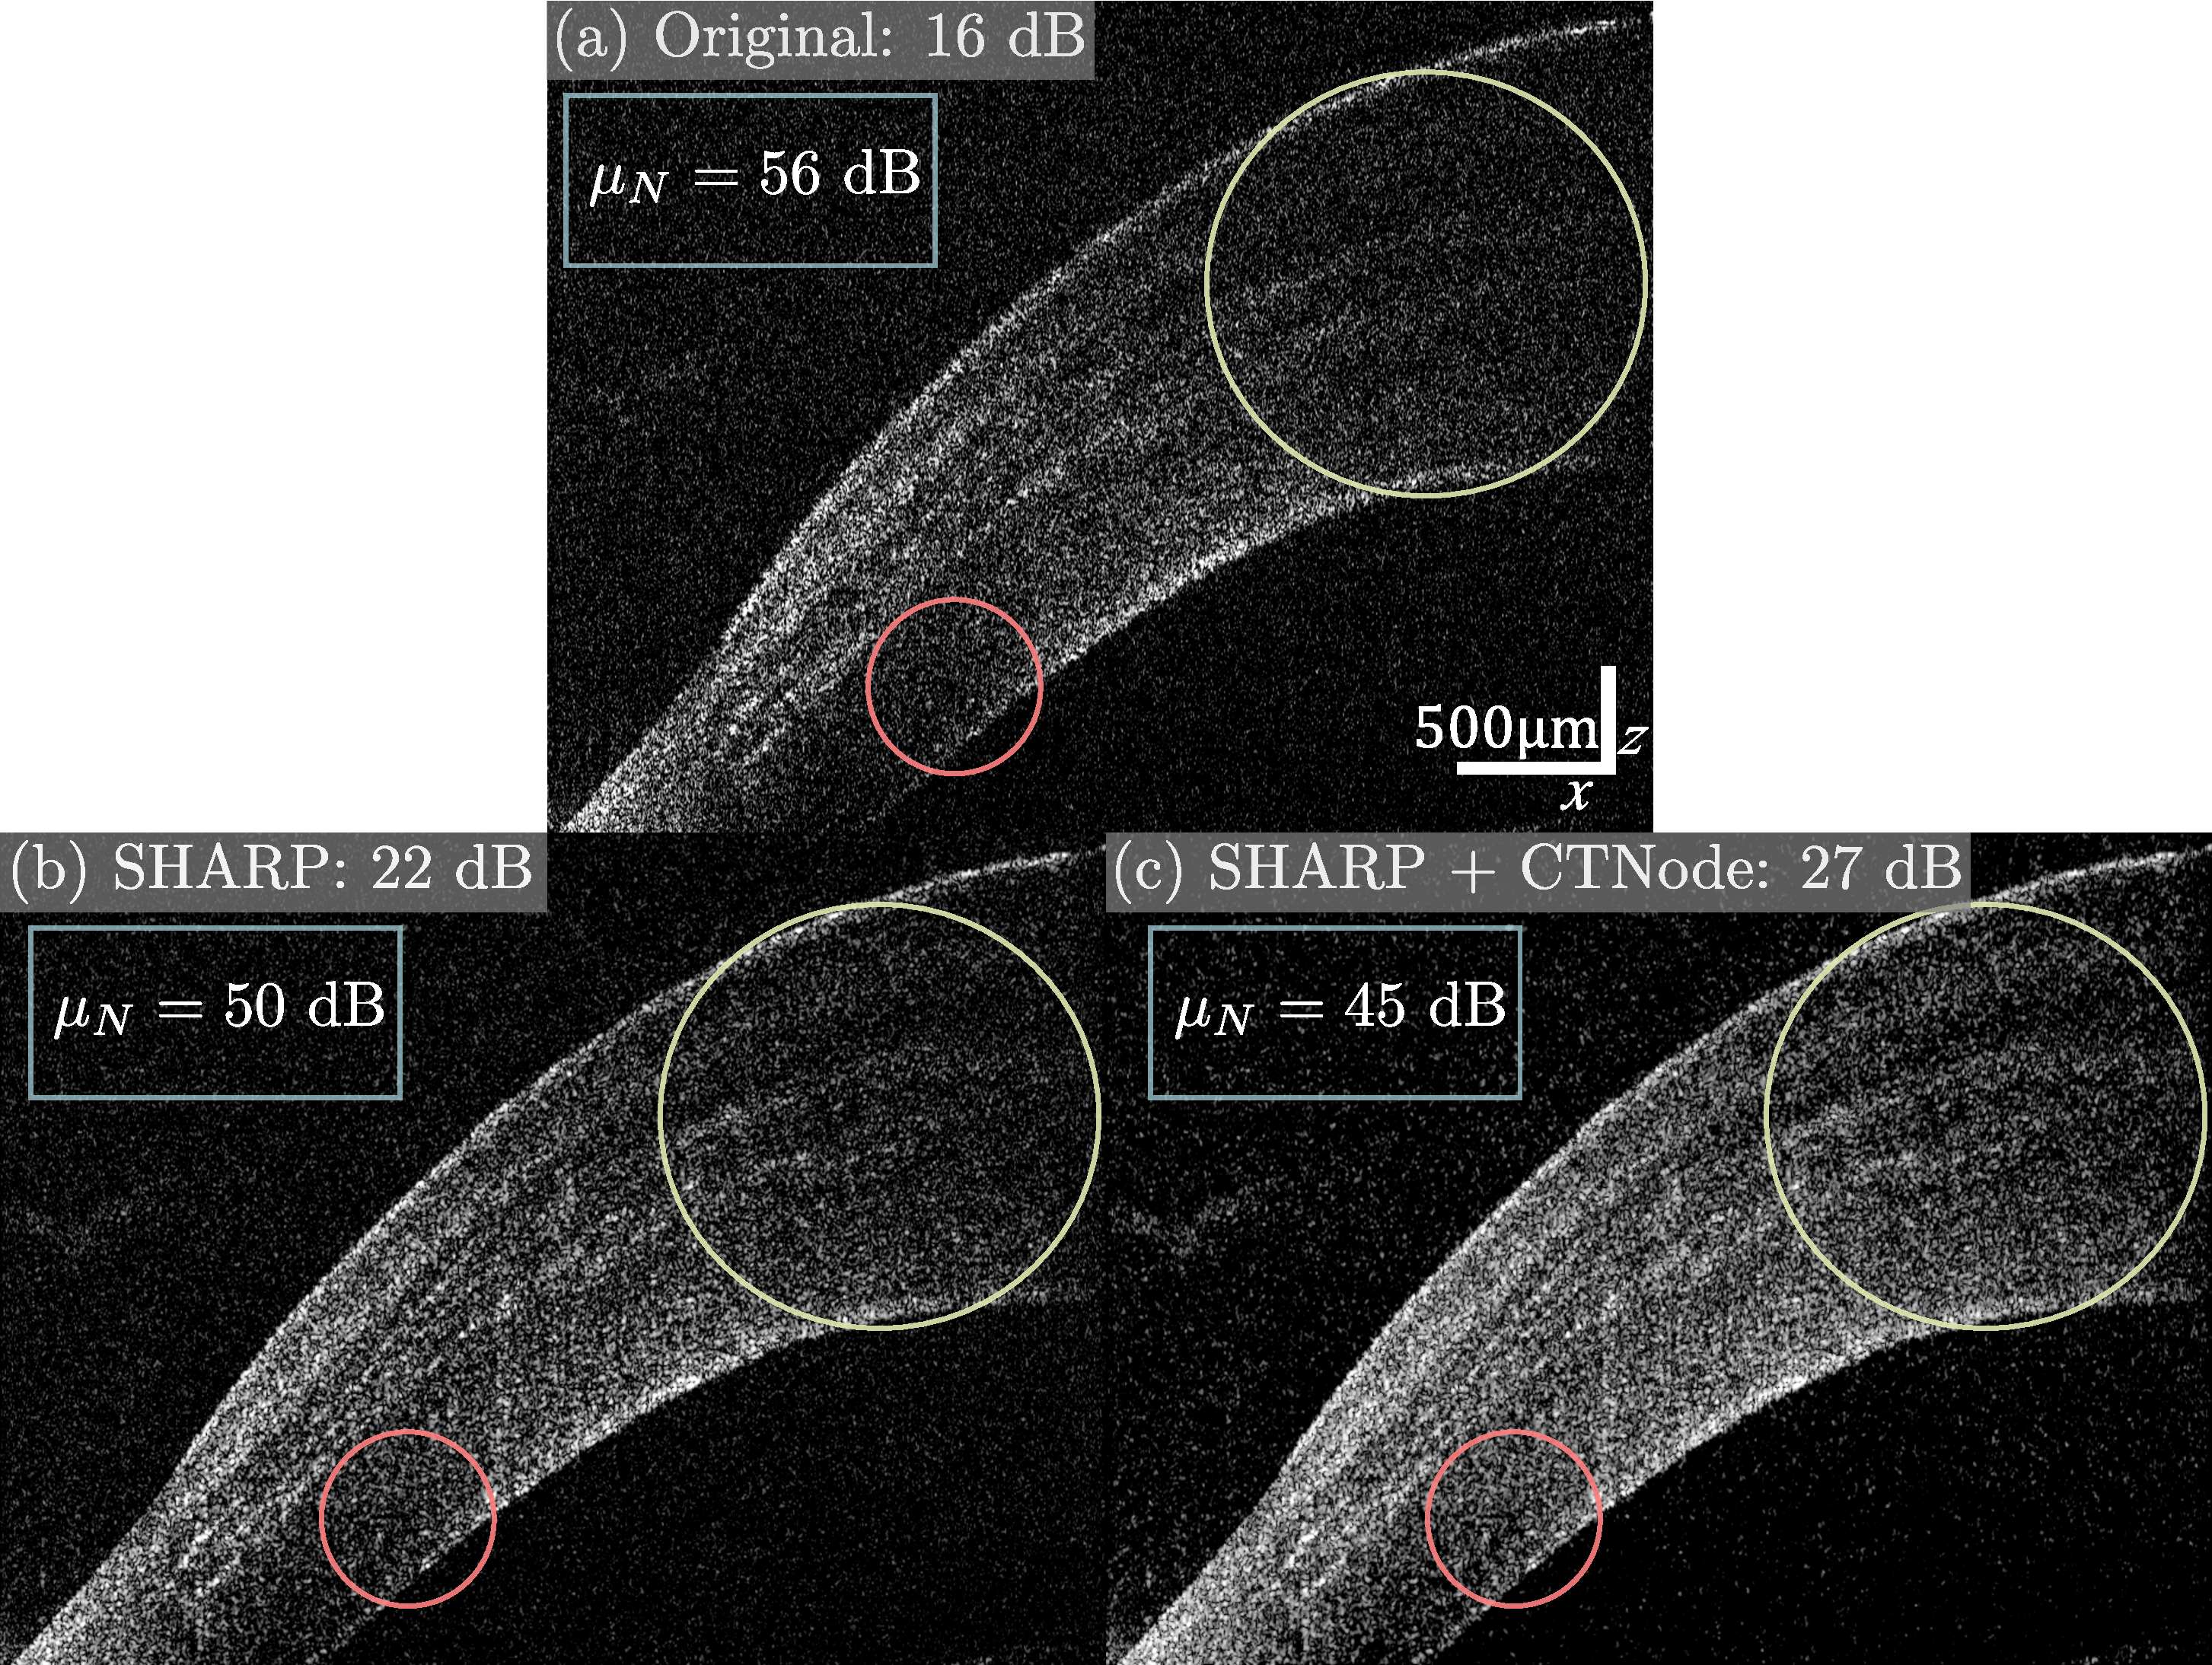
\includegraphics[width=\textwidth]{Figures/Results/ASImaging-CTNode.pdf}
	\caption[Combination of SHARP and CTNode in anterior segment of excised swine eye.]{Combination of SHARP and CTNode in anterior segment of excised swine eye. B-scan images: (a) original, (b) after SHARP and (c) after subsequent CTNode. Number in the label of each image corresponds to its dyanmic range.}
	\label{fig:ASImaging_CTNode}
\end{figure}

\FloatBarrier

Apart from the correction of defocus, the image after SHARP and CTNode presents an overall improvement in contrast of low and medium-SNR regions, such as the regions enclosed in circles of Fig.~\ref{fig:ASImaging_CTNode}(c) where signal is more clearly visualized than their counterparts in Figs.~\ref{fig:ASImaging_CTNode}(a) and (b). A notable side effect is that contrast of high intensity signal seems to be reduced, as a consequence of the asymmetric extension of dynamic range: the noise floor level is decreased but the signal strength is not increased, but in fact it is technically impossible to increase signal strength computationally. Despite that, the beneficial effect of noise reduction is more significant, for instance the corneal stroma, presents a better contrast after CTNode than in the original image where stroma exhibits a signal just above noise floor level because of its relative low back-scattering and the negative effect of aberrations. This suggests that CTNode has potential to improve the visualization of tissue with low to medium SNR signal by means of noise reduction. Another important aspect is that no resolution loss was observed after CTNode, which is particularly relevant for SHARP given that it is desired to maintain the resolution improvement provided by correction of aberrations.

\subsection{Correction of anisotropic defocus in the cornea}\label{sec:CorneaImaging}

The optical properties of the tissue being imaged affect the propagation of the probe beam, and in particular this may give rise to spatial variations of the focal position which means that the focus does not follow a plane but a deformed surface, depending on sample geometry. The cornea possess a curved surface and an index of refraction different to air and these features combined produce a variation of focal position across the field of view following a smooth curvature, resulting in a \textit{focal curve} rather than a focal plane. This phenomenon, encountered mainly in high-NA systems, demands spatially-varying aberrations correction.

To demonstrate correction of anisotropic defocus in the cornea, the SSOCT system was equipped with a scan lens producing an effective $e^{-2}$ beam diameter of 9~$\mu$m in a Rayleigh range of 97~$\mu$m. The excised swine eye was imaged around the cornea apex, tilting the sample to avoid signal saturation due to specular reflection near to the apex, which ultimately resulted in a even greater spatial variation of focal position. An ROI of 350 samples per A-lines, 1536 A-lines per B-scan and 1024 B-scans was selected, covering a lateral field of view of 5$\times$3.3~mm$^2$ in an axial ranging of 2~mm in air. It has been found that a better aberration correction is obtained if window-based CAO is applied after global CAO in each 1D aberration correction step, possibly because global correction serves as an initial estimate to aberration correction which is then improved locally with window-based correction. In this case, only Legendre polynomial $P_2$ was employed and, for window-based SHARP, the window size was set to 128$\times$128 (0.4$\times$0.4~mm$^2$).

Figure~\ref{fig:ConrealImaging} shows an \textit{en face} view of the original tomogram and after correction of aberrations with global and window-based SHARP. In this case, the optimum filter reduced noise floor level by 6~dB but contrast improvement is not evident because the dynamic range of original image in Fig.~\ref{fig:ConrealImaging}(a) was adjusted to match the contrast of the SHARP image in Fig.~\ref{fig:ConrealImaging}(b) for comparison purposes. Displayed \textit{en face} planes are located at a depth within the corneal stroma, marked by yellow line in original B-scan image in Fig.~\ref{fig:ConrealImaging}(c), presenting very dense signal but also fine structures that are significantly blurred in the original tomogram, whereas after SHARP they appear sharper given the improvement of lateral resolution, as noted when comparing the insets that show zoomed regions of the images.

\begin{figure}[htb!]
	\centering
	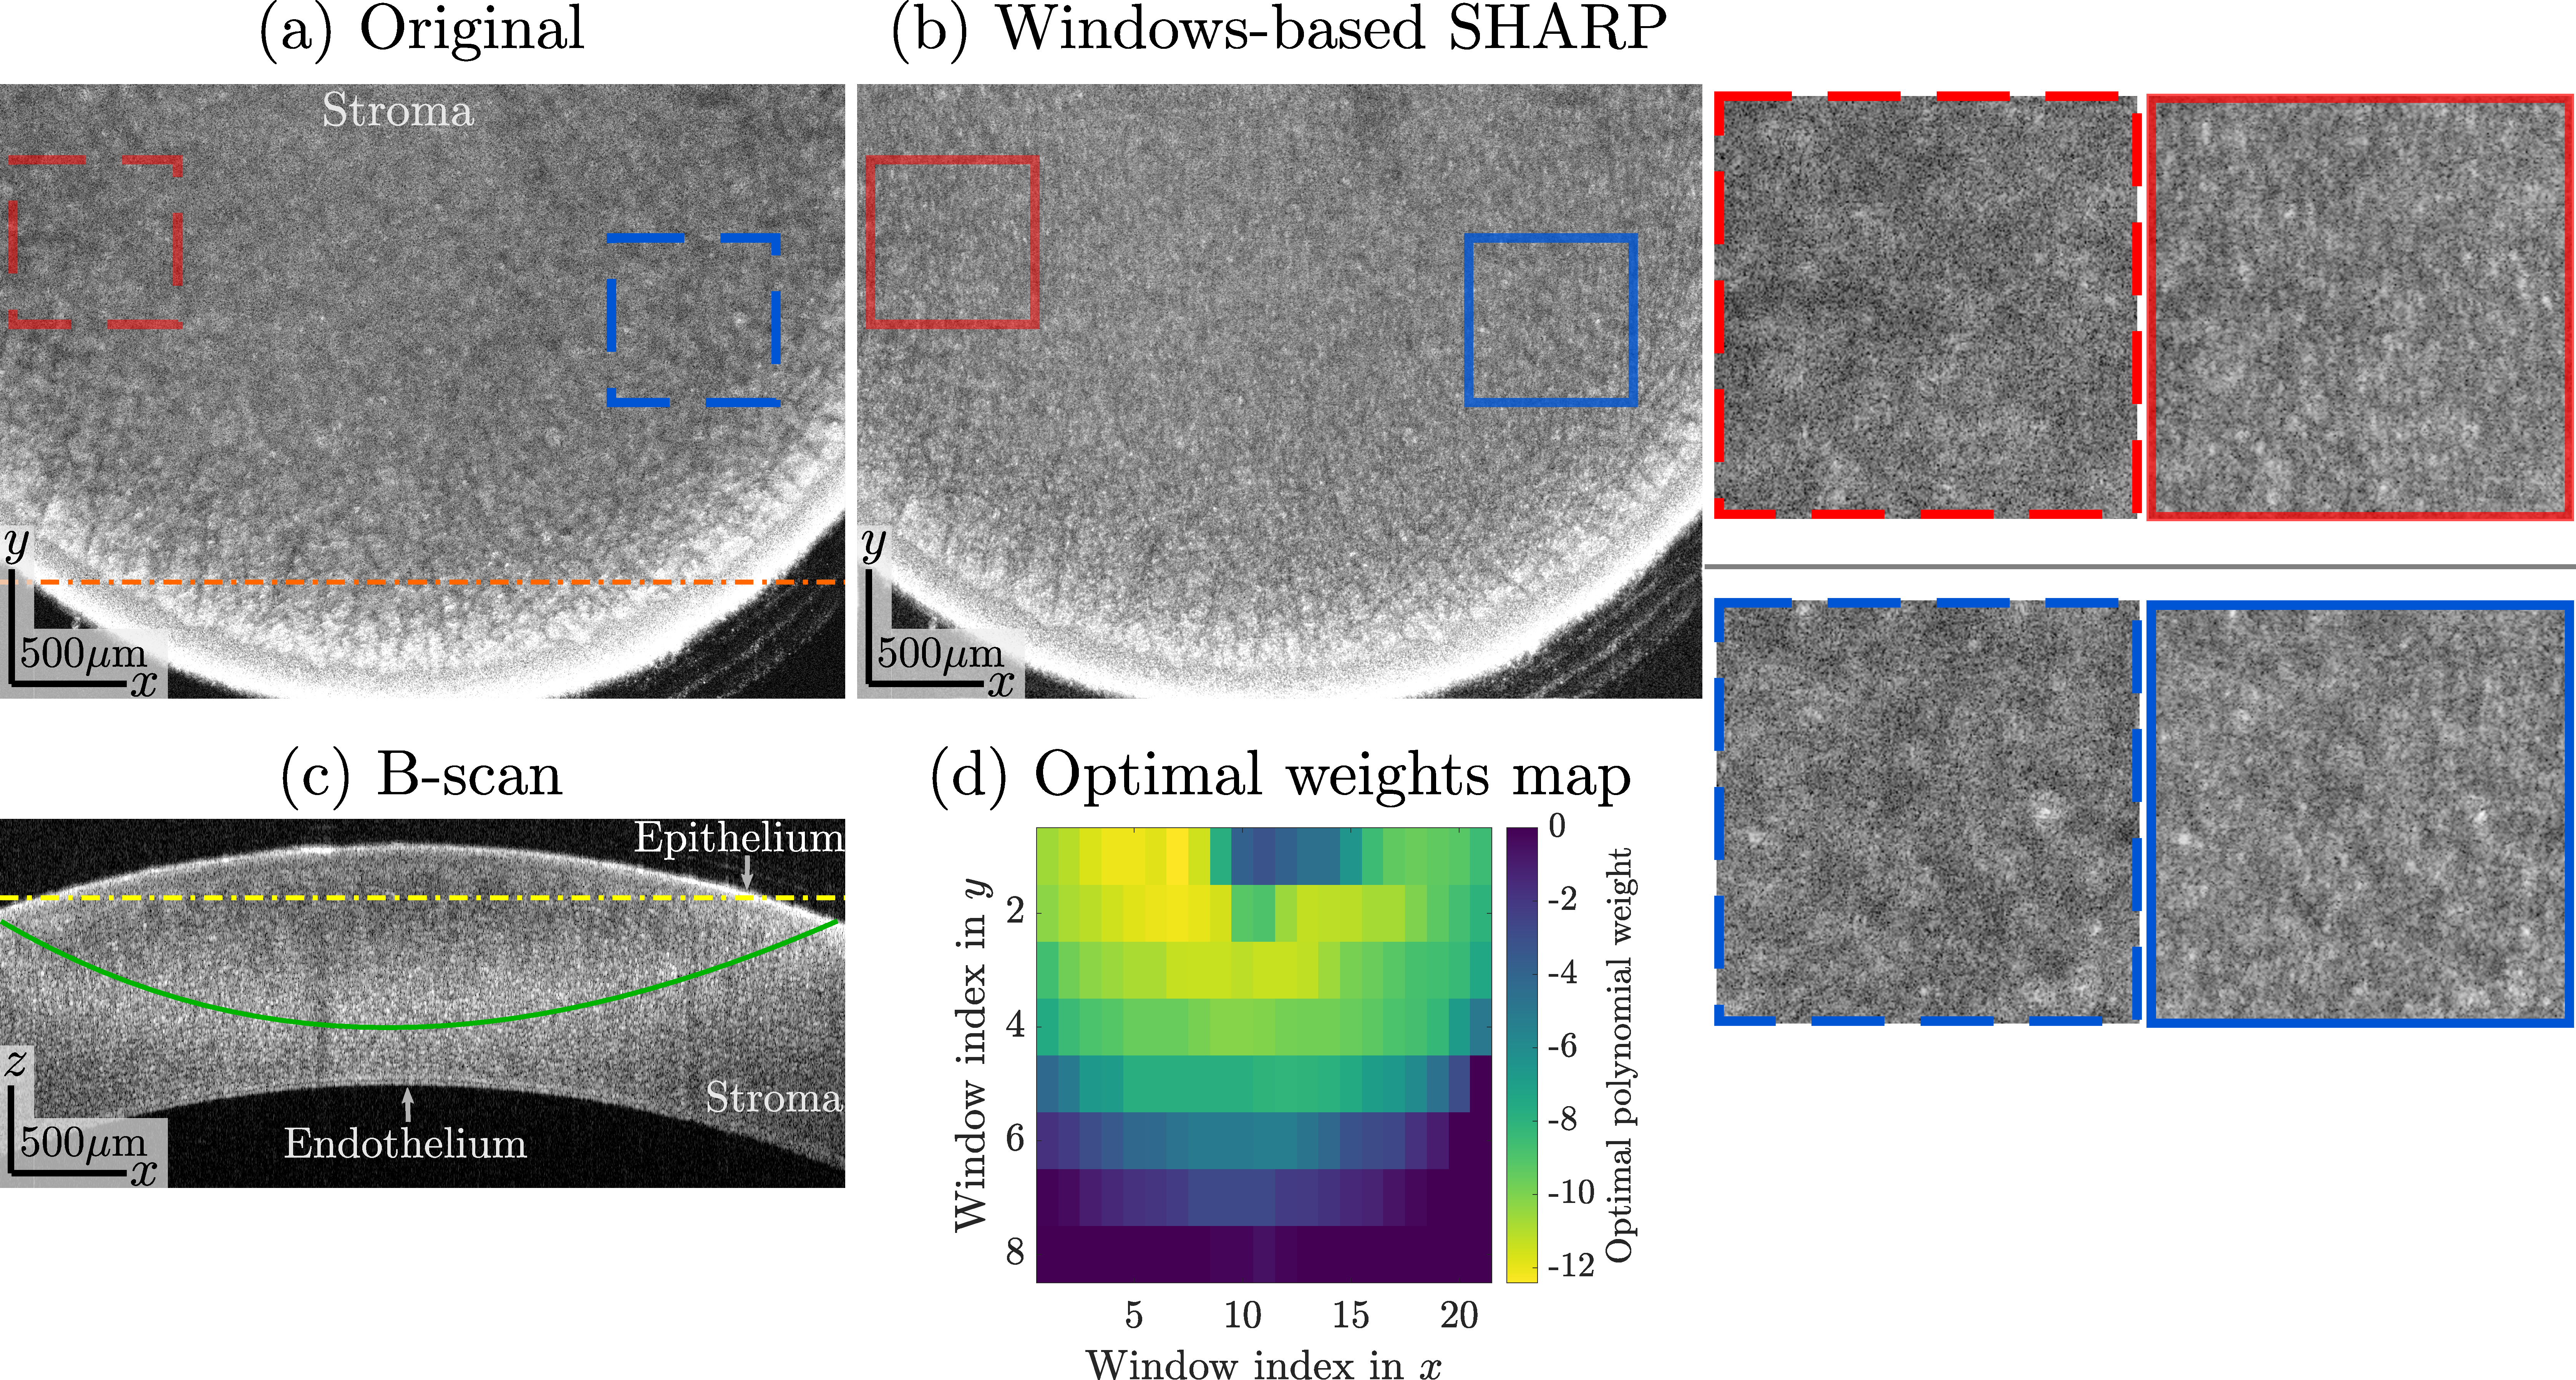
\includegraphics[width=\textwidth]{Figures/Results/CorneaImaging.pdf}
	\caption[Application of SHARP in cornea of excised swine eye.]{Application of SHARP in cornea of excised swine eye. \textit{En face} views of (a) original tomogram and (b) after SHARP and window-based SHARP, located at depth marked by yellow dashed line in the original B-scan in (c), that at the same time corresponds to the location marked by orange dashed-line in (a). (d) Two-dimensional map of optimal 
	weights for all windows found for correction along $x$ of \textit{en face} plane in (b).}
	\label{fig:ConrealImaging}
\end{figure}

In practical terms, the depth of field can be often identified in cross-sectional views as a bright intensity band because signal inside the depth of field is intrinsically stronger than outside. This way, it is possible to roughly determine the position of the focus as the center of this bright band, which in the B-scan view of Fig.~\ref{fig:ConrealImaging}(c) follows a curve instead of a plane, as marked by green line, indicating that indeed the location of the focus varies with lateral position, resulting in a focal curve. This effect can be also inferred from the two-dimensional map in Fig.~\ref{fig:ConrealImaging}(d) that shows the optimal weights determined for each window for the \textit{en face} plane in Fig.~\ref{fig:ConrealImaging}(b), which resemble the cornea curvature, instead of being constant across all windows as expected if the correction were purely global.

\FloatBarrier

\section{Complex noise reduction in human posterior segment imaging \textit{in vivo}}

The posterior segment of the eye is rich in structures that support the normal operation of the eye, such as the retinal nerve fiber layer, the photoreceptors layer and the choroid~\cite{Drexler2015_Retinal}. In general, these structures present high back-scattering that vary between them allowing a readily visual identification in intensity-contrast image. However, choroid and sclera typically present a lower signal, specially the sclera, given that they are at deep depths where signal strength is greatly affected by tissue absorption and the high reflectance of precedent layers like the retinal pigment epithelium. Measurement of the choroid thickness has been of great interest for diagnosis and study of pathologies~\cite{Yiu2014_Characterization}, and this requires to identify the choroid/sclera (C/S) junction in order to reliable identify the choroid and measure its thickness, but this task is difficult given the relatively low contrast of the C/S junction. 

An additional experimental validation of CTNode was performed, aiming to reduce noise in retinal imaging to improve contrast of structures, including the C/S junction. The posterior segment of a healthy subject was imaged using a retinal system described in~\cite{Braaf2018_Complex}. This SSOCT system is based on a VCSEL wavelength-swept source (Axsun Technologies, Inc., MA, USA) with an A-line repetition rate of 100~kHz and a spectral bandwidth of 91~nm centered at wavelength 1040~nm for an axial resolution of 10~$\mu$m in air. The system has a modified commercial ophthalmic interface (Heidelberg Engineering, Germany), that provides a diffraction-limited spot-size of 18~$\mu$m on the retina, with an integrated scanning laser ophthalmoscope (SLO) to track motion of the subject's eye by analyzing motion-induced affine image transformations compared to a pre-acquired reference SLO image, and then motion correction is translated to the control wave-forms of the galvanometers scanners of the SSOCT system on-the-fly in order to follow eye motions during the acquisition. Additionally, a reference reflection in a separated arm of the sample arm is available for 2D phase stabilization.

The acquired tomogram consisted in 2048 depth samples, 1024 A-lines per B-scan and 1024 B-scans, from which an ROI of 820$\times$960$\times$768 was extracted for processing. Phase was stabilized using the reference reflection~\cite{Vakoc2005_Phaseresolved}. Furthermore, residual motion was observed despite the use of the motion tracking system, mostly slow-frequency motion, that was corrected using intra-B-scan bulk motion correction as described in Section~\ref{sec:MotionCor}. Phase stabilization and motion correction enabled the use of 3D search and similarly windows, which otherwise would be restricted to 2D or 3D with limited performance. CTNode was applied using search and similarity windows of size 15$\times$15$\times$15 and 3$\times$3$\times$3, respectively, and $h=0.12$.

B-scan views of the original tomogram and after CTNode are shown in Figures~\ref{fig:RetinalCTNode}(a) and (b), corresponding to the cross-section marked by red dashed lines in \textit{en face} views shown in Figs~\ref{fig:RetinalCTNode}(d) and (e). In the original image, signal decays smoothly in the choroid making it difficult to identify the C/S junction. Application of CTNode provided a noise level reduction of 6~dB, allowing to increase the dynamic range of the image from 38~dB to 44~dB. This improvement is visualized in the medium-SNR layers in between the retinal nerve fiber layer and the photoreceptors layer that present a high contrast with respect to noise floor level, but the contrast between layers seems to be reduced, due to the side-effect of CTNode mentioned before. Anyhow, the interest is not to visualize high intensity layers, but more importantly the signal in the choroid that is more clearly identified from the sclera which is masked by the noise level, possibly improving a further determination of C/S junction. Plot in Fig.~\ref{fig:RetinalCTNode} shows A-line profiles of the original and CTNode tomogram, at location marked by blue dashed lines in Figs.~\ref{fig:RetinalCTNode}(a) and (b). Signal within the green line have high intensity and thus reduction of noise is inconsequential, but for low signal regions within the orange line, such as the sclera, noise reduction is perceived as a decrease in signal intensity. Finally, Figs.~\ref{fig:RetinalCTNode}(d) and (e) show \textit{en face} views of the original and CTNode tomograms at depths marked by purple dashed lines in the B-scans. Signal around the optic disk is very homogeneous in the original \textit{en face} because SNR is low and noise dominates, instead, CTNode \textit{en face} view displays a transition in signal intensity from the choroid to the sclera. 

\begin{figure}[htb!]
	\centering
	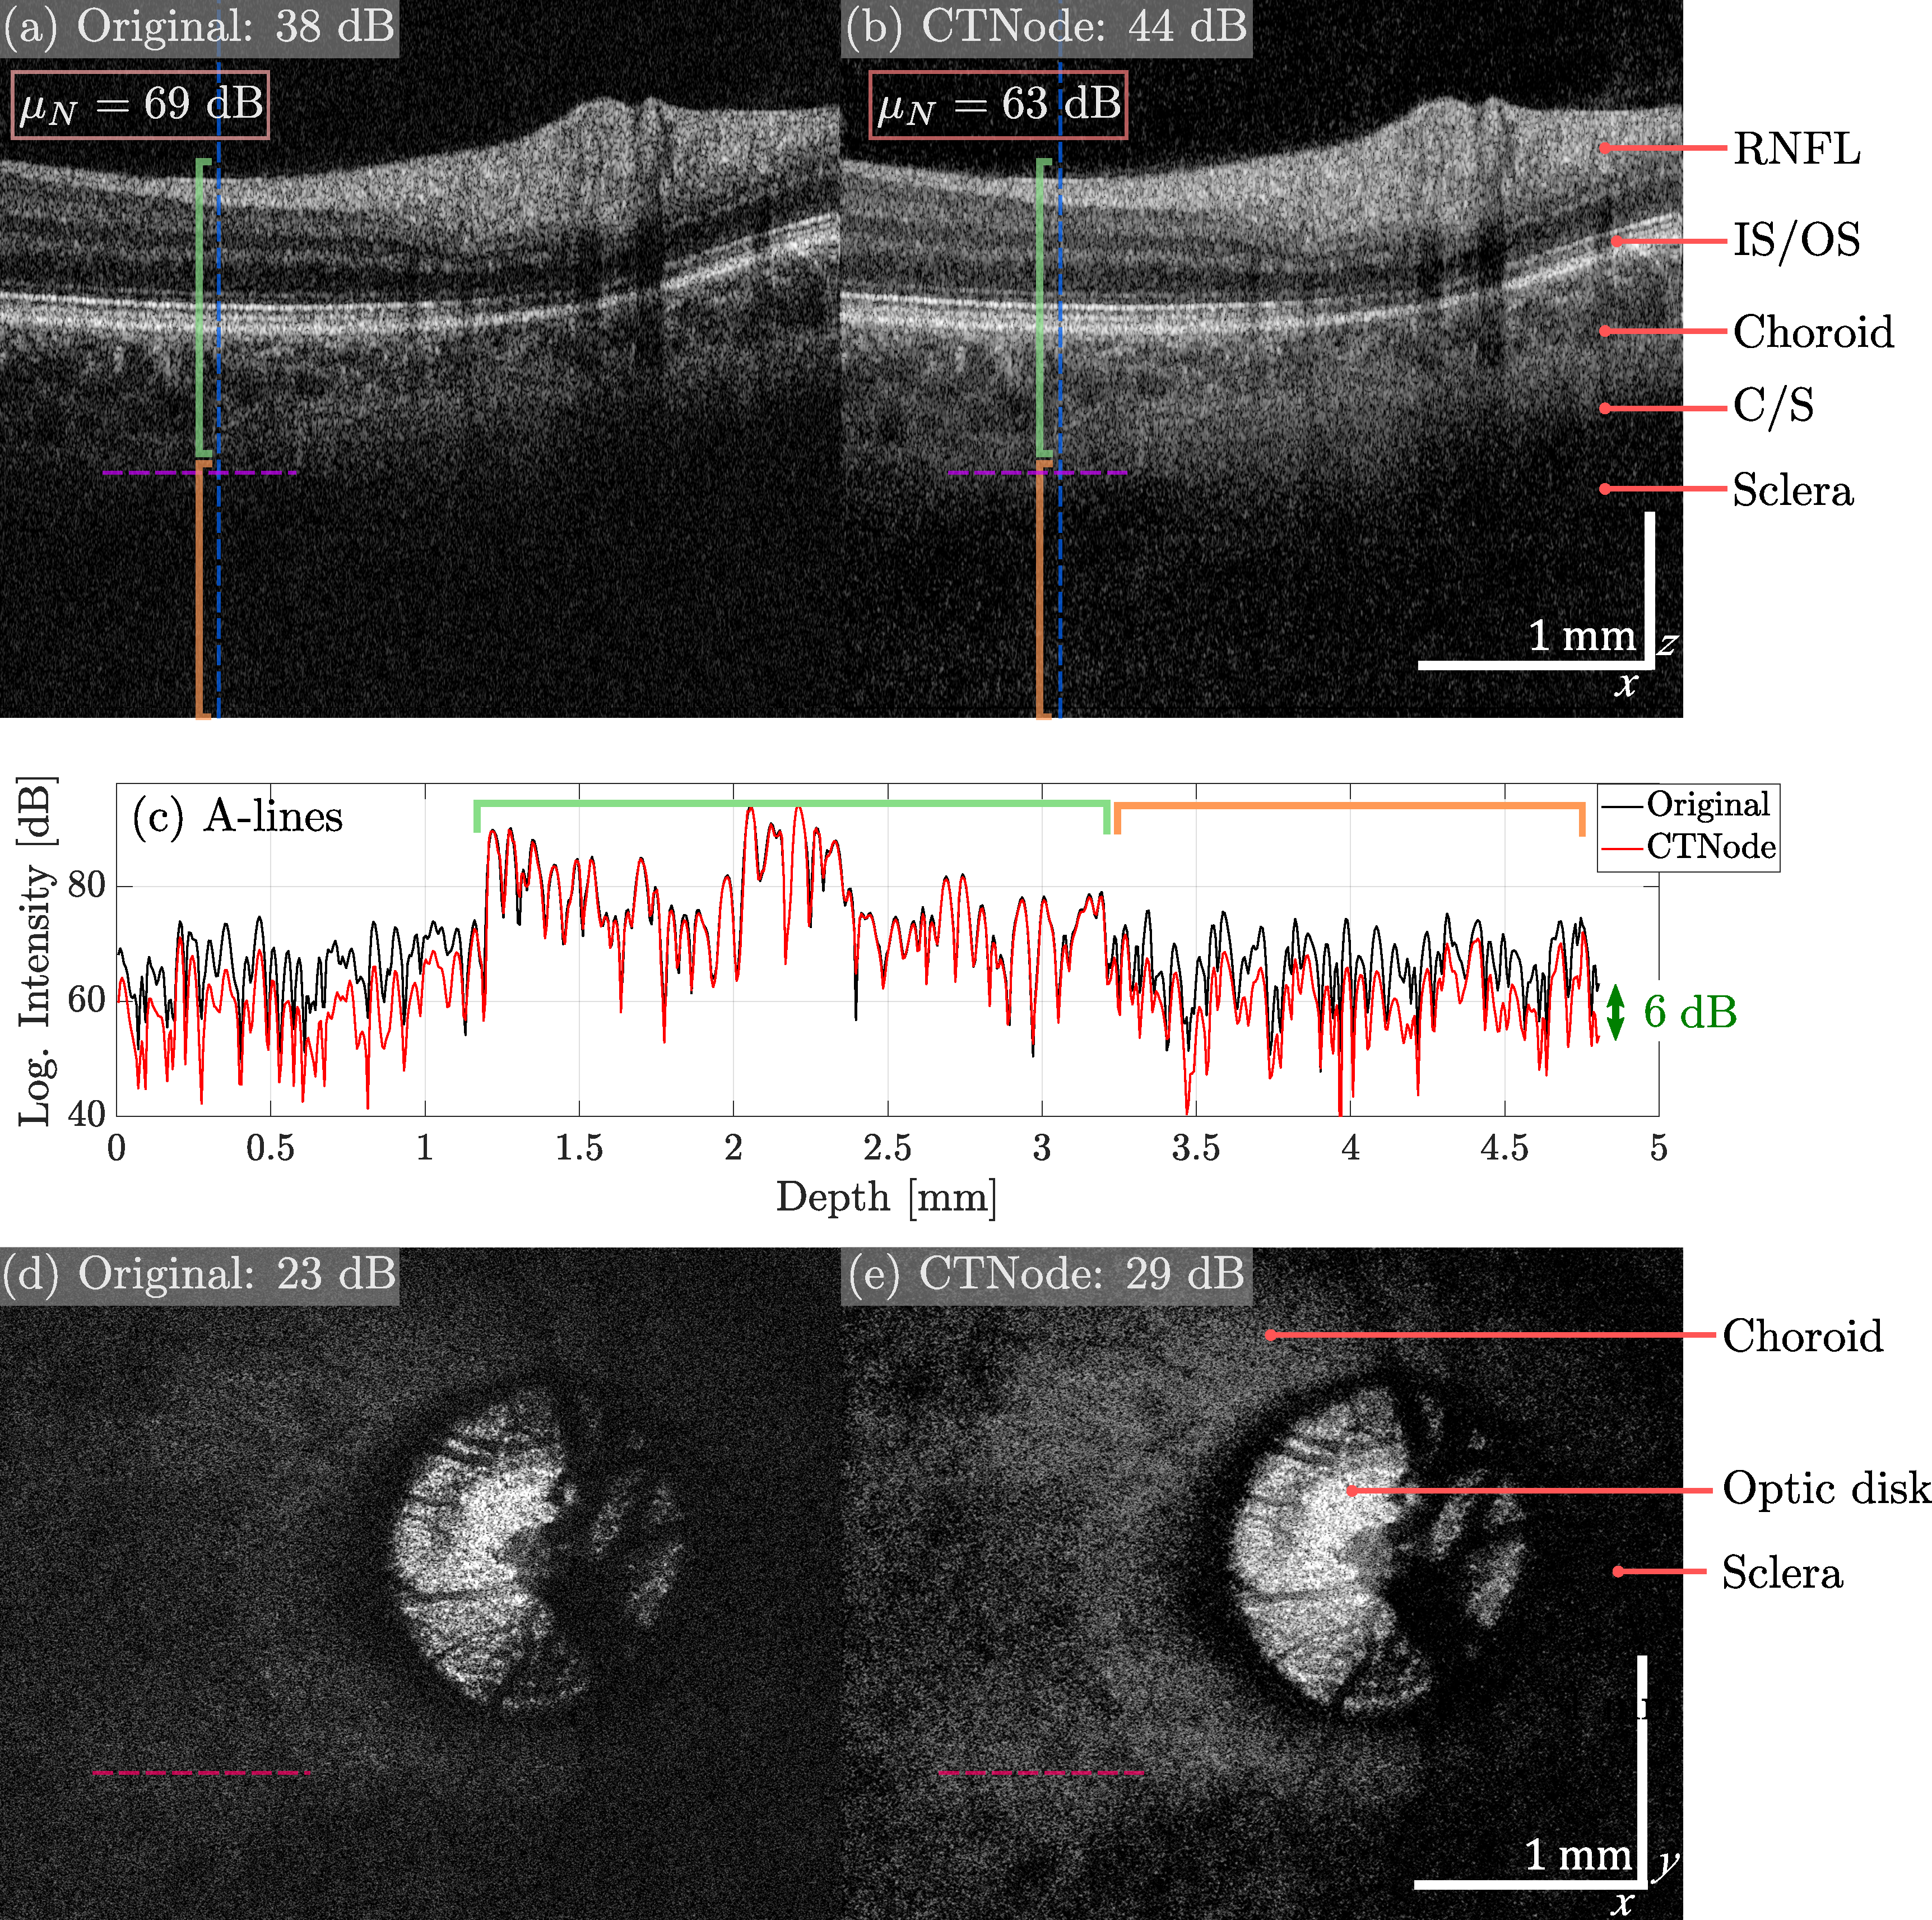
\includegraphics[width=\textwidth]{Figures/Results/RetinalCTNode.pdf}
	\caption[Reduction of noise with CTNode in retinal imaging \textit{in vivo}.]{Reduction of noise with CTNode in retinal imaging \textit{in vivo}. B-scan views: (a) original and (c) after CTNode, corresponding to the plane marked by red dashed lines in \textit{en face} views: (d) original and (e) after CTNode, at depth marked by purple dashes lines in (a) and (b). (c) A-line profile of original and CTNode tomograms at locations marked by blue lines in (a) and (b). RNFL: retinal nerve fiber layer, IS/OS: inner and outer photoreceptors segment junction, C/S: Choroid/sclera junction. }
	\label{fig:RetinalCTNode}
\end{figure}

\FloatBarrier

\section{Endoscopic imaging \textit{in vivo}}

To access internal tissue like coronary artery~\cite{Brezinski1996_Imaging} or gastrointestinal tract~\cite{Isenberg2003_Gastrointestinal} with endoscopic OCT, the scanner system composed of the galvo mirrors is replaced by a catheter that is inserted into the tissue lumen to guide light and to image internal structures. Light propagates inside the catheter through an optic fiber until the output tip, then it is focused by a gradient-index (GRIN) lens and finally it is reflected by a mirror or a prism by 90$^\circ$,  perpendicular to the lumen direction towards the interior of tissue~\cite{Hu2015_Optical}, as illustrated in Figure~\ref{fig:CatheterSchematic}. To scan the sample, A-lines are acquired while the catheter is being rotated by an external or internal actuator, providing B-scans of axial and \textit{azimuthal} axes, and additionally the catheter is pulled-back along the \textit{longitudinal} axis during the scanning to acquire multiple frames producing volumetric data. The probe is enclosed in a protective transparent tube to provide stability and prevent mechanical damage arising from the direct contact of the optics and the tissue, but this element induces astigmatism given its cylindrical geometry~\cite{Hu2015_Optical, Wang2012_Numerical, Xi2009_Highresolution}  . As a consequence, the beam spot size in the longitudinal axis is different to that in the azimuthal axis, furthermore, the working distance in B-scan plane $d_x$ becomes larger than in longitudinal plane $d_y$~\cite{Wang2012_Numerical}, as depicted in Fig.~\ref{fig:CatheterSchematic}

\begin{figure}[htb!]
	\centering
	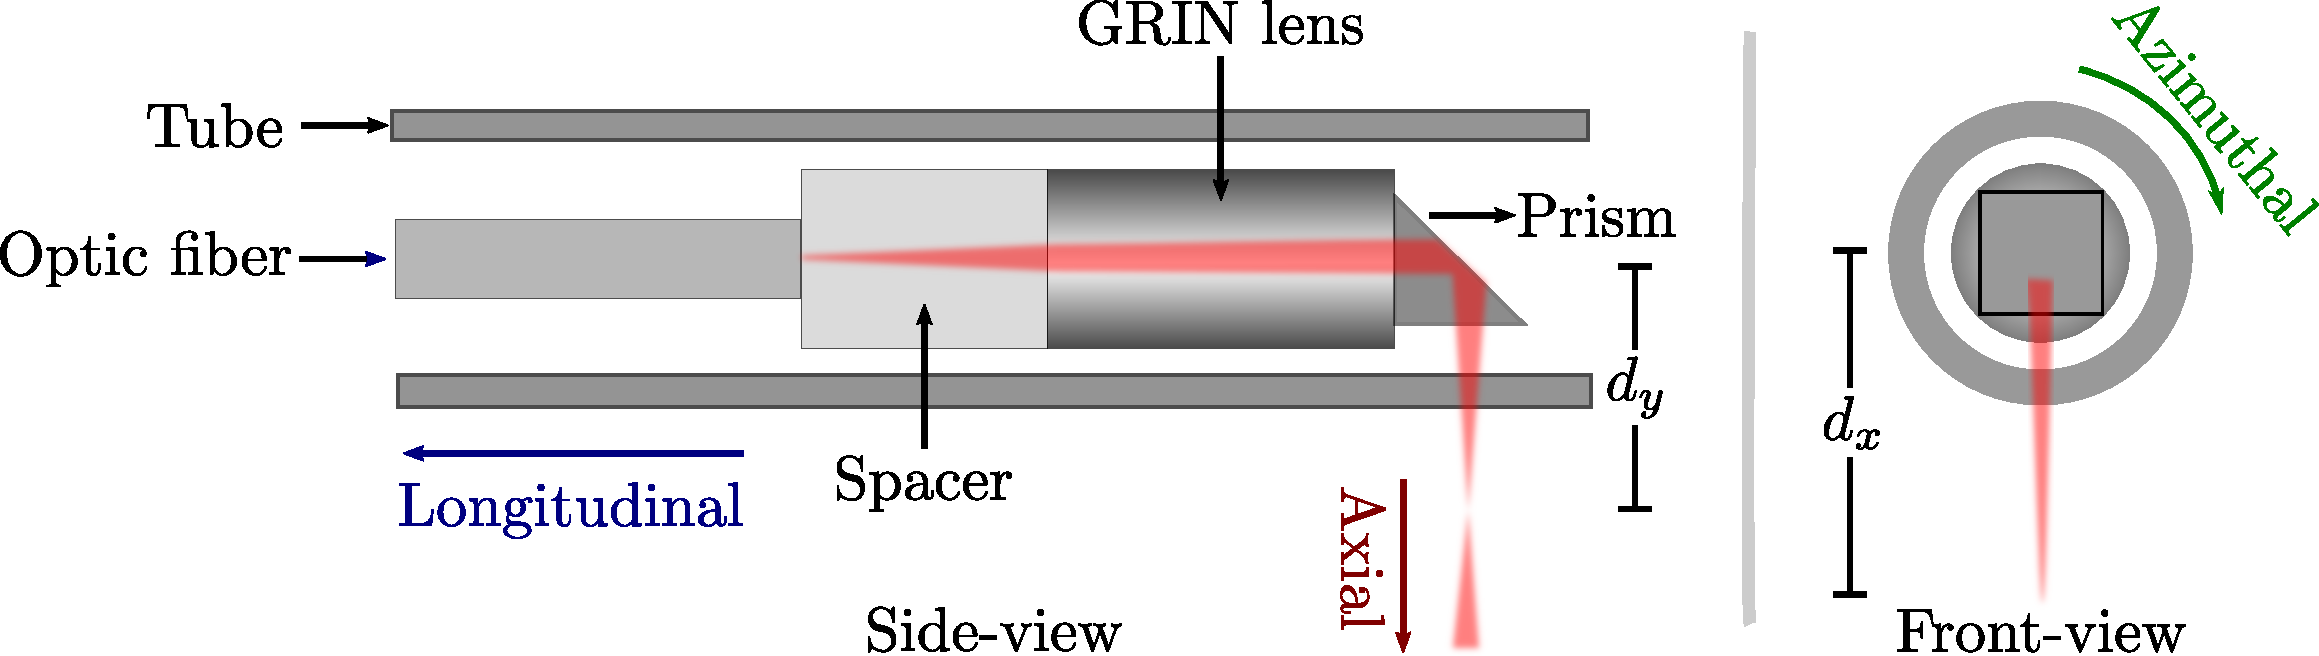
\includegraphics[width=.9\textwidth]{Figures/Results/CatheterSchematic.pdf}
	\caption[Schematic of a catheter for endoscopic OCT imaging.]{Schematic of the side-view and the front-view a catheter for endoscopic OCT imaging.}
	\label{fig:CatheterSchematic}
\end{figure}

In raster scan systems, it is possible to adjust the distance between the scan lens and the sample to position the region of interest inside the the imaging range, however, because the catheter-sample distance is fixed in endoscopic imaging, the working distance is a key feature in practical scenarios. For instance, a long working distance is required in esophageal imaging, whereas a short one is demanded in coronary artery imaging~\cite{Wang2012_Numerical}, thus optical design of catheter has become important~\cite{Hu2015_Optical, Xi2009_Highresolution, Kang2010_Endoscopically}, in order to produce astigmatism-free catheters with the desired working distance. Computational refocusing has the potential to facilitate optical design of catheters by correcting the negative effect of astigmatism and providing focused images across a larger depth of field without need of changing the working distance of the catheter.

The pullback of the catheter is typically performed such that the longitudinal sampling is often very sub-Nyquist and unevenly sampled, also, severe motion artifacts appear due to the probe rotation and the pullback, and for these reasons longitudinal axis is unsuitable for numerical aberration correction, thus only 1D refocusing is possible in endoscopic imaging, which is indeed possible with SHARP-$x$, computing only $\tilde{S}^{\text{1D}}$ in Eq.~\eqref{eq:SHARP}.

To demonstrate 1D operation of SHARP in endoscopic OCT for defocus and/or astigmatism correction, pullbacks of the airway of a swine were acquired \textit{in vivo} with a non-$k$-clocked catheter-based OCT system (NinePoint Medical Inc., Bedford, MA) having a 50~kHz polygon-based wavelength-swept source with $90$~nm $10$-dB bandwidth at central wavelength $1310$~nm and $e^{-2}$ beam diameter of $2w_0=40~\mu$m with Rayleigh range $z_R=1$~mm in air. SHARP was applied using $P_2$ only and TNode despeckling was performed afterwards using similarity and search windows of 5$\times$5$\times$0 and 31$\times$31$\times$5 pixels, respectively, and filtering parameters $h_0 = 0.06$ and $h_1 = 0.03$. Figure~\ref{fig:CatheterImaging} presents original and SHARP B-scans after TNode at two pullback positions showing an ROI of 450$\times$750~px$^2$ above the focal plane, which is located close to the lower edge of the images, making that structures near to the catheter wall appear blurred. Although 1D correction alone is more limited than 2D correction, SHARP-$x$ still provides an enhancement for depths $z>z_R$. In particular, debris in the mucus layer, located just below the catheter wall, is brought into focus as seen in the insets. This result suggests that SHARP-$x$ could improve endoscopic imaging when there is no fixed probe-tissue working distance, such as in airway and intravascular imaging, by combining long working distance catheters with SHARP to provide focal resolution in an extended range.

\begin{figure}[htb!]
	\centering
	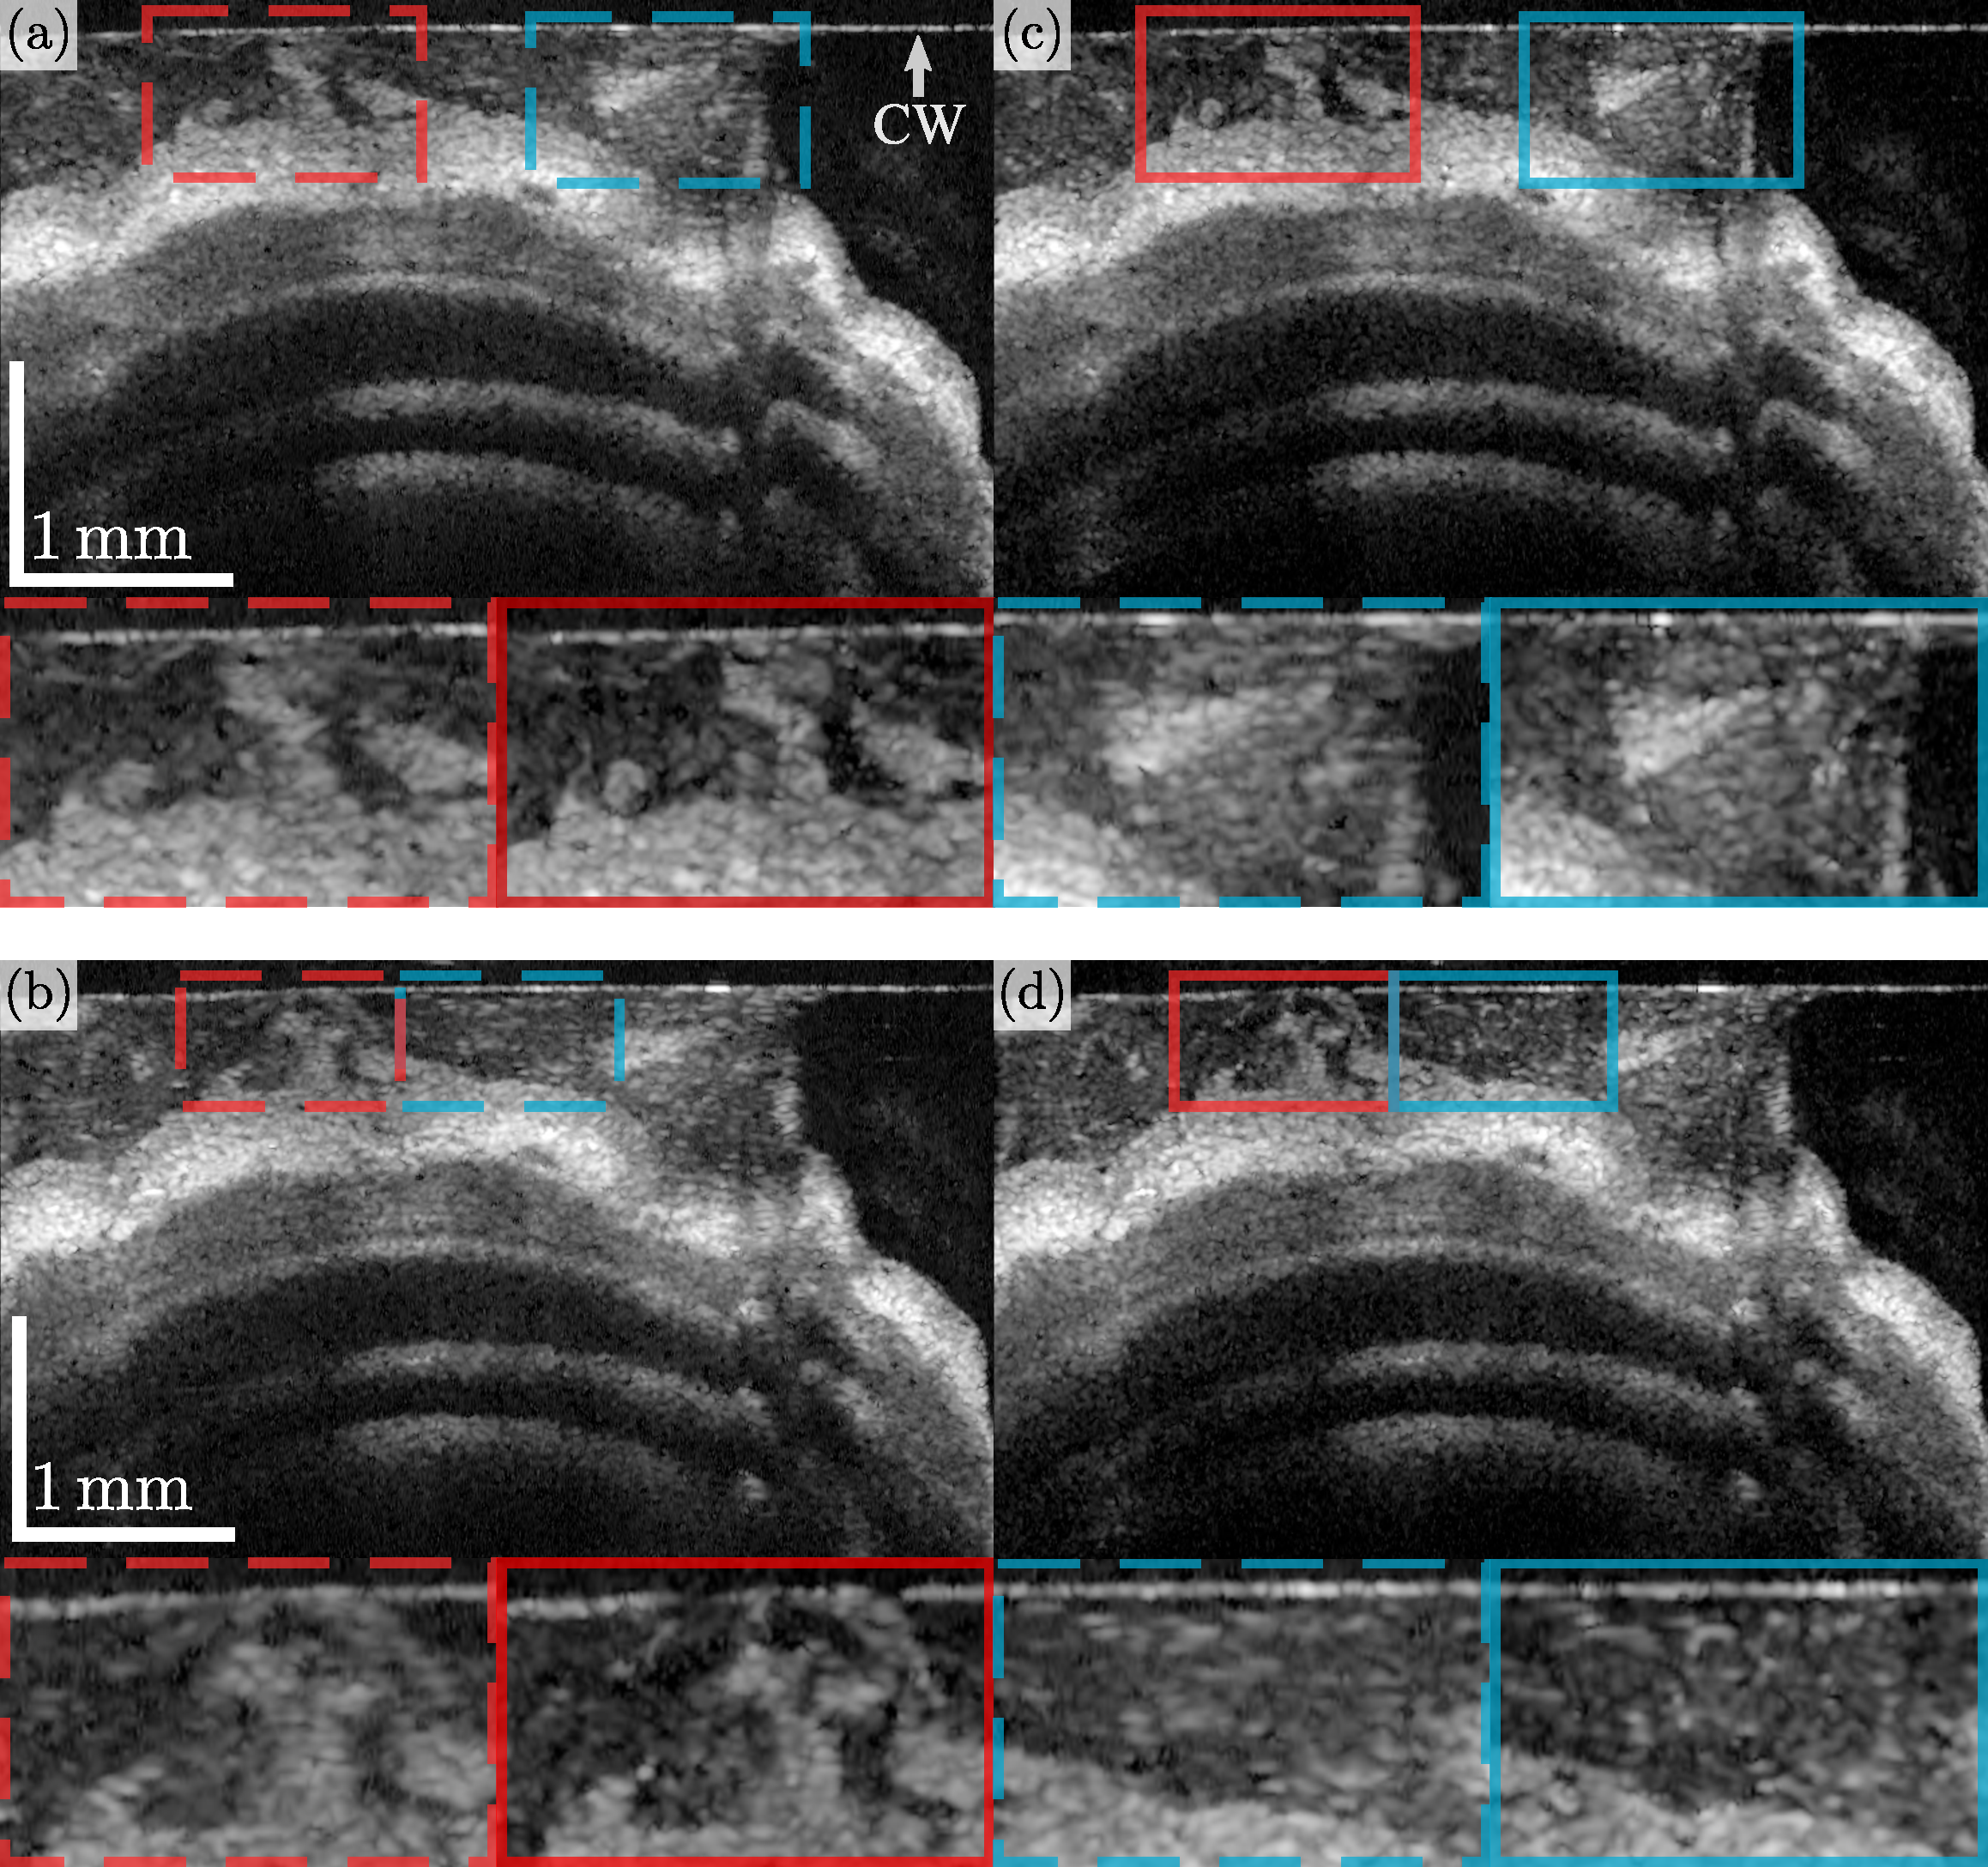
\includegraphics[width=.9\textwidth]{Figures/Results/CatheterImaging.pdf}
	\caption[Application of SHARP in endoscopic imaging of swine airway \textit{in vivo}.]{Application of SHARP in endoscopic imaging of swine airway \textit{in vivo}. B-scan views: (a)-(b) original and (c)-(d) SHARP-$x$. CW: catheter wall.}
	\label{fig:CatheterImaging}
\end{figure}

\FloatBarrier

\section{Skin imaging \textit{in vivo}}

OCT offers readily observation of features of the skin such as stratum corneum, sweat ducts and dermal/epidermal junction and promises to offer key information for quick reliable diagnosis, in applications where avoiding skin biopsy is desirable~\cite{Holmes2015_OCT}. To demonstrate operation of SHARP in skin imaging, a tomogram of a human hand dorsal surface was imaged \textit{in vivo} with the focal plane above the sample surface, using the same system and configuration used for the proof of concept experiment but selecting now an ROI of 500 samples per A-line, 512 A-lines per B-scan and 256 B-scans. The sample was imaged around the metacarpophalangeal joint, which presents an inhomogenous surface inducing spatial variations of defocus that make insufficient to correct the entire lateral FoV globally. Therefore, windows-based SHARP was applied using windows of size 64$\times$64~px$^2$. Although the hand of the subject was resting on a platform, small, low-frequency motion is evidenced in the tomogram, possibly dominated by heartbeat. Intra-B-scan motion correction was performed after phase stabilization along $x$, obtaining axial and lateral shifts of the order of a few micros, as shown in Figure~\ref{fig:SkinImaging}(a). The small shifts can be observed in the  blue inset aside Fig.~\ref{fig:SkinImaging}(d), which do not appear after correction. TNode despeckling was applied to display all images using similarity and search windows of 7$\times$7$\times$7 and 15$\times$15$\times$15 pixels, respectively, and filtering parameters $h_0 = 0.07$ and $h_1 = 0.01$.

\begin{figure}[htb!]
	\centering
	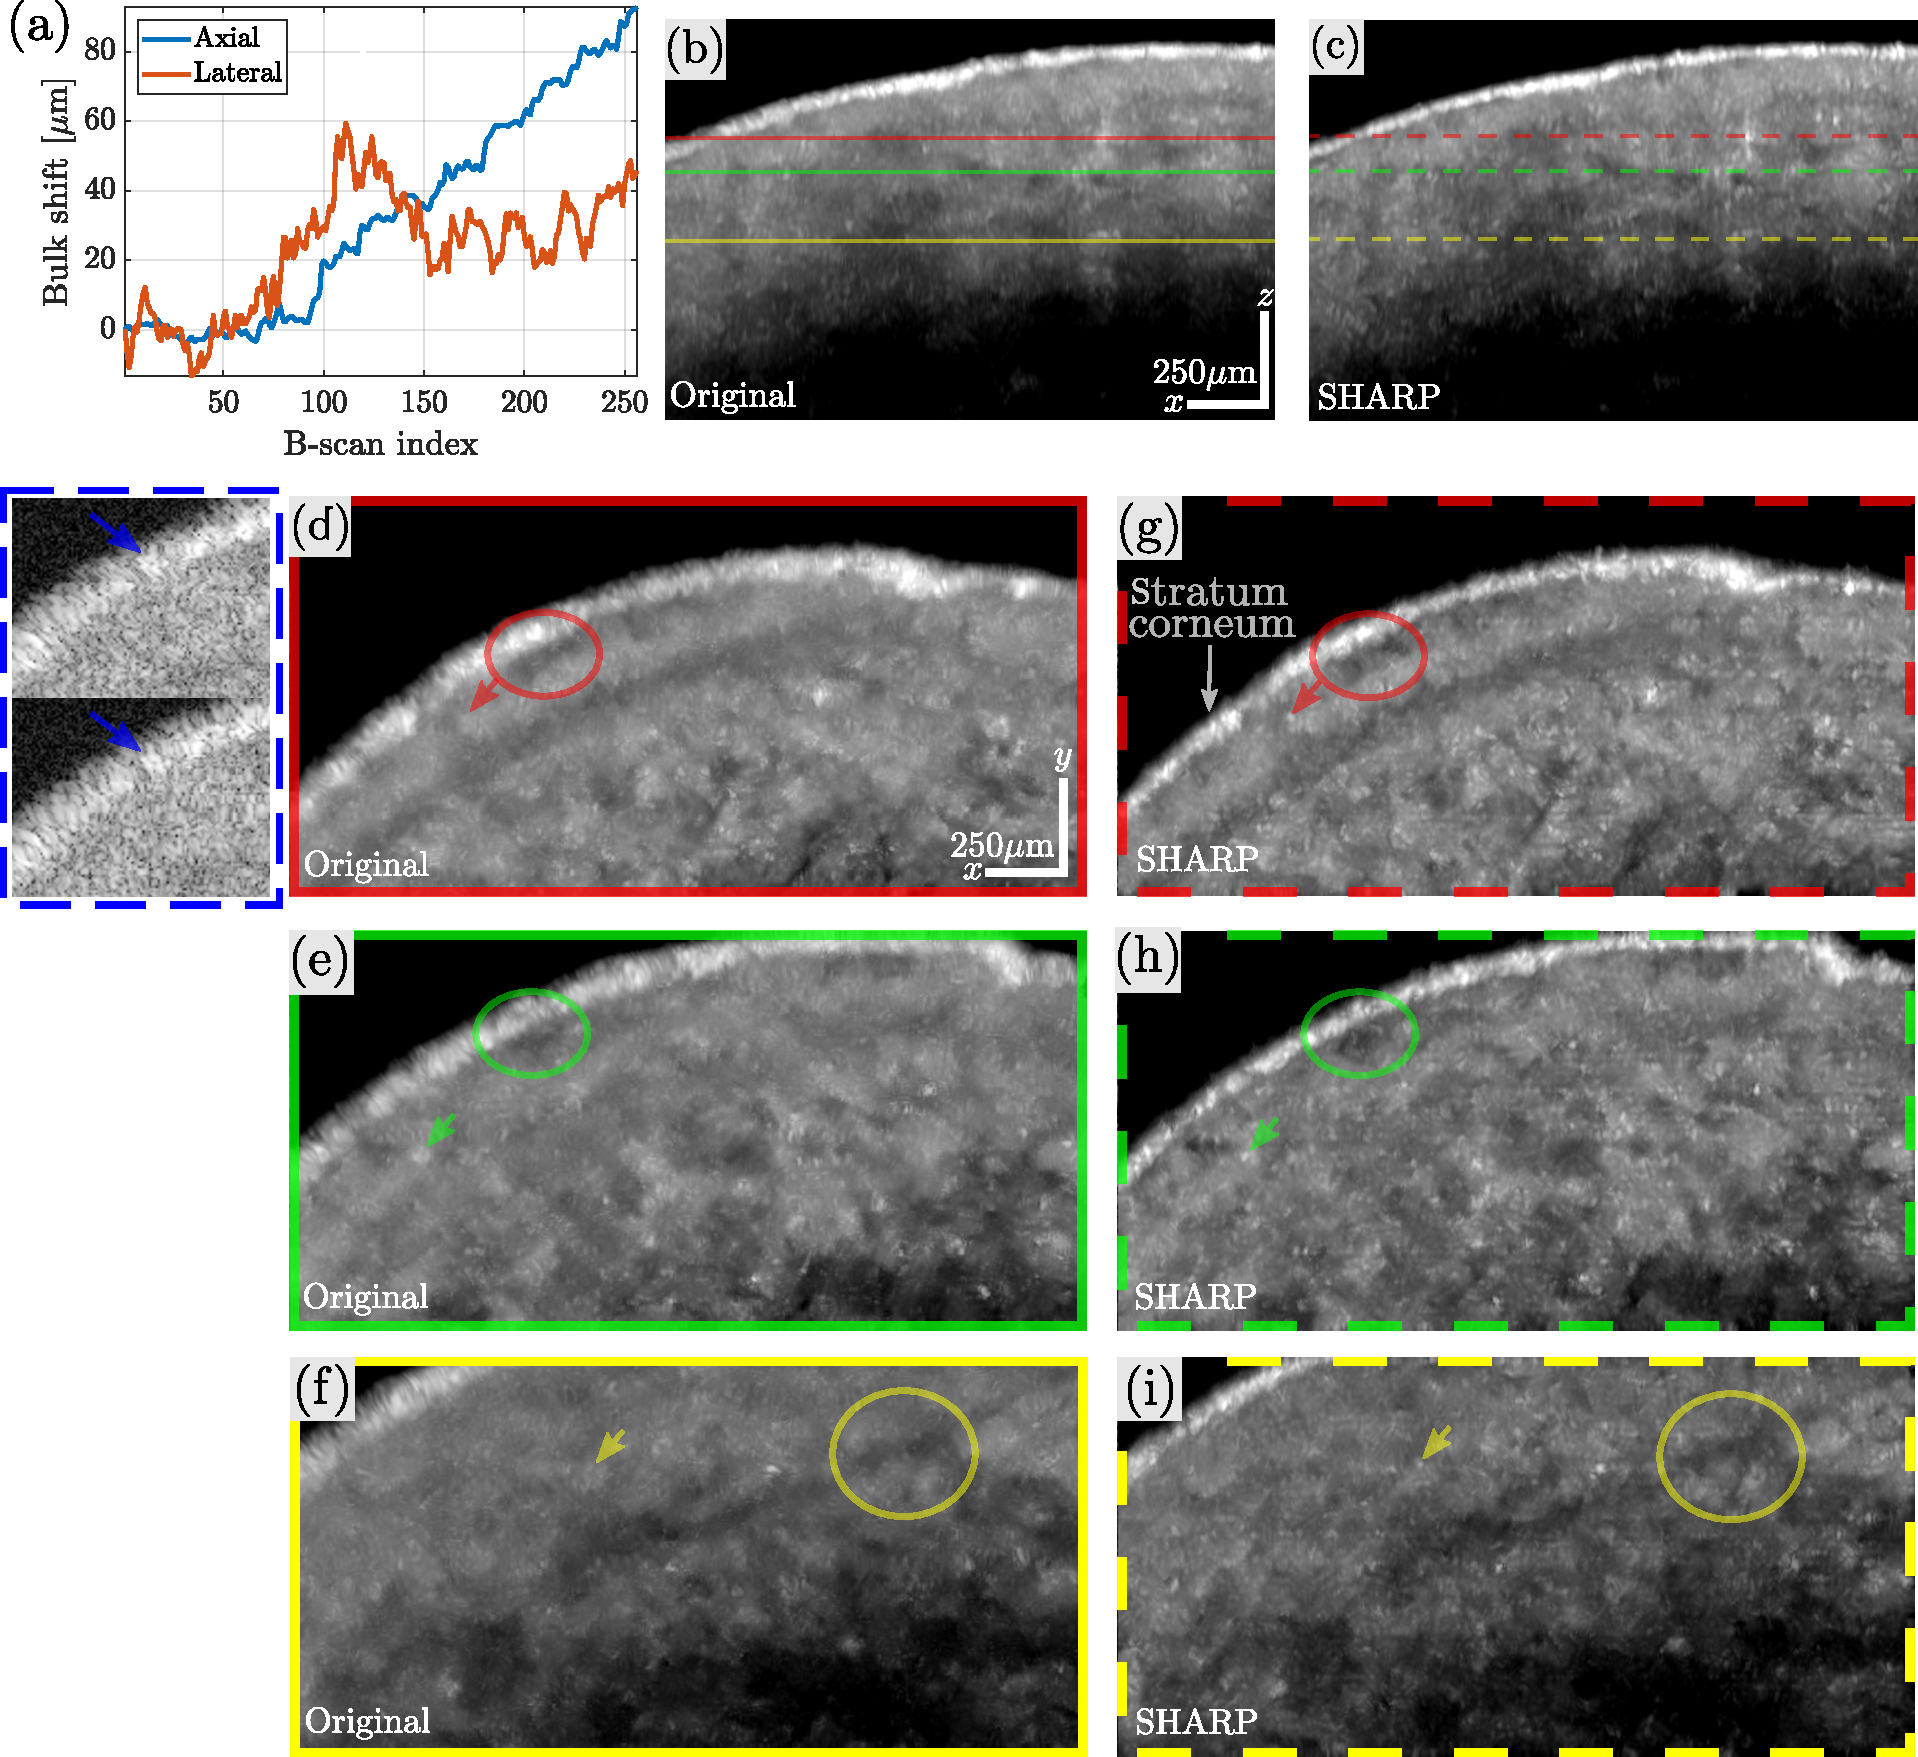
\includegraphics[width=\textwidth]{Figures/Results/SkinImaging.pdf}
	\caption[Application of SHARP in skin imaging \textit{in vivo}]{Application of SHARP in human skin imaging \textit{in vivo}. (a) Axial and lateral shifts determined in motion correction. B-scan views: (b) before and (c) after windows-based SHARP. \textit{En face} views at different depths marked in (b) and (c): (d)-(f) original tomogram and (g)-(i) windows-based SHARP tomogram. Blue inset corresponds to a small \textit{en face} ROI before (top) and after (bottom) motion correction.}
	\label{fig:SkinImaging}
\end{figure}

Figure~\ref{fig:SkinImaging} shows three different \textit{en face} planes of the motion-corrected and SHARP tomograms at depths indicated by the lines on B-scan views in Figs.~\ref{fig:SkinImaging}(b) and (c). Original \textit{en face} views in Figs.\ref{fig:SkinImaging}(e)-(g) present strong blurring, particularly towards the tissue surface, whereas corrected \textit{en faces} in Fig.\ref{fig:SkinImaging}(h)-(j) present sharper features with reduction of smearing that allows to visualize small details throughout the FoV with better contrast. For instance, fine bright structures appear after refocusing such as those marked with arrows and differences in contrast between tissues is observed clearer, like those  enclosed with circles. Most notably, the stratum corneum is brought to focus showing a reduction of the visual thickness. Major limitation of CAC techniques in dermatology is the presence of high multiple scattering that is particularly stronger in skin than in other tissues, frustrating aberration correction for depths deep into the tissue, however, skin imaging is in general shallow given the relatively high light absorption of skin tissue. These successful results demonstrate the ability of SHARP to refocus \textit{in vivo} addressing not only phase noise but complex amplitude shifts as well.

\section{Computational refocusing in polarization-sensitive OCT}

To demonstrate the possibility to preform computational refocusing in PS-OCT, a dataset of the anterior segment of an excised porcine eye was acquired. As seen in the previous experiments, anterior segment imaging is an attractive application that could benefit from computational refocusing due to its surface topography, which posses a long axial extension that precludes the use of medium-NA, and in particular for PS-OCT there is a potential clinical interest in high-resolution polarimetric parameters of tissue in this application~\cite{Li2020_Vectorial}. The sample was imaged around the limbus with the focal plane located deep into the tissue targeting the trabecular mesh-work. The dataset was acquired with the polygon-based SSOCT system and configuration used for the experiment in Section~\ref{sec:CorneaImaging}, but this time activating an integrated electro-optic modulator used to modulate the two illumination orthogonal polarization states between alternating A-lines in the fast scan axis. The acquired spectra were splitted into 5 spectral windows for the spectral binning processing with an overlap of 66~\% between them. The tomogram contains 1024 B-scans and 1024 A-lines with 1024 depth samples, with a pixel size of 3.3~$\mu$m in lateral axes and $6~\mu$m in the axial axis in air, from which different regions of interest were selected to process. SHARP was applied following the procedure proposed for polarization-sensitive imaging, using only defocus correction since it is the dominant aberration in the experiment, and then the Stokes vector components were spatially-averaged by using a Gaussian kernel with $e^{-2}$ diameter 13$\times$13 $\mu$m$^2$ (4$\times$4 px$^2$) oriented in the lateral axes only.

The analysis was centered on the limbal region, depicted in the B-scan of Figure~\ref{fig:PSOCT_int}(a), where the short vertical yellow line represents the length of the confocal parameter. The focus is visualized approximately in the middle of the yellow box. This configuration is representative of medium-NA imaging of the limbus, where the axial extent of the tissue makes impossible to have the whole ROI in focus. Figs.~\ref{fig:PSOCT_int}(b) and (c) show \textit{en face} intensity views before and after SHARP, respectively, at the depth indicated by the dotted line in Fig.~\ref{fig:PSOCT_int}(a). The intensity after SHARP exhibits a higher contrast and better resolution given the correction of defocus and the effect of the optimum filter.

\begin{figure}[htb!]
	\centering
	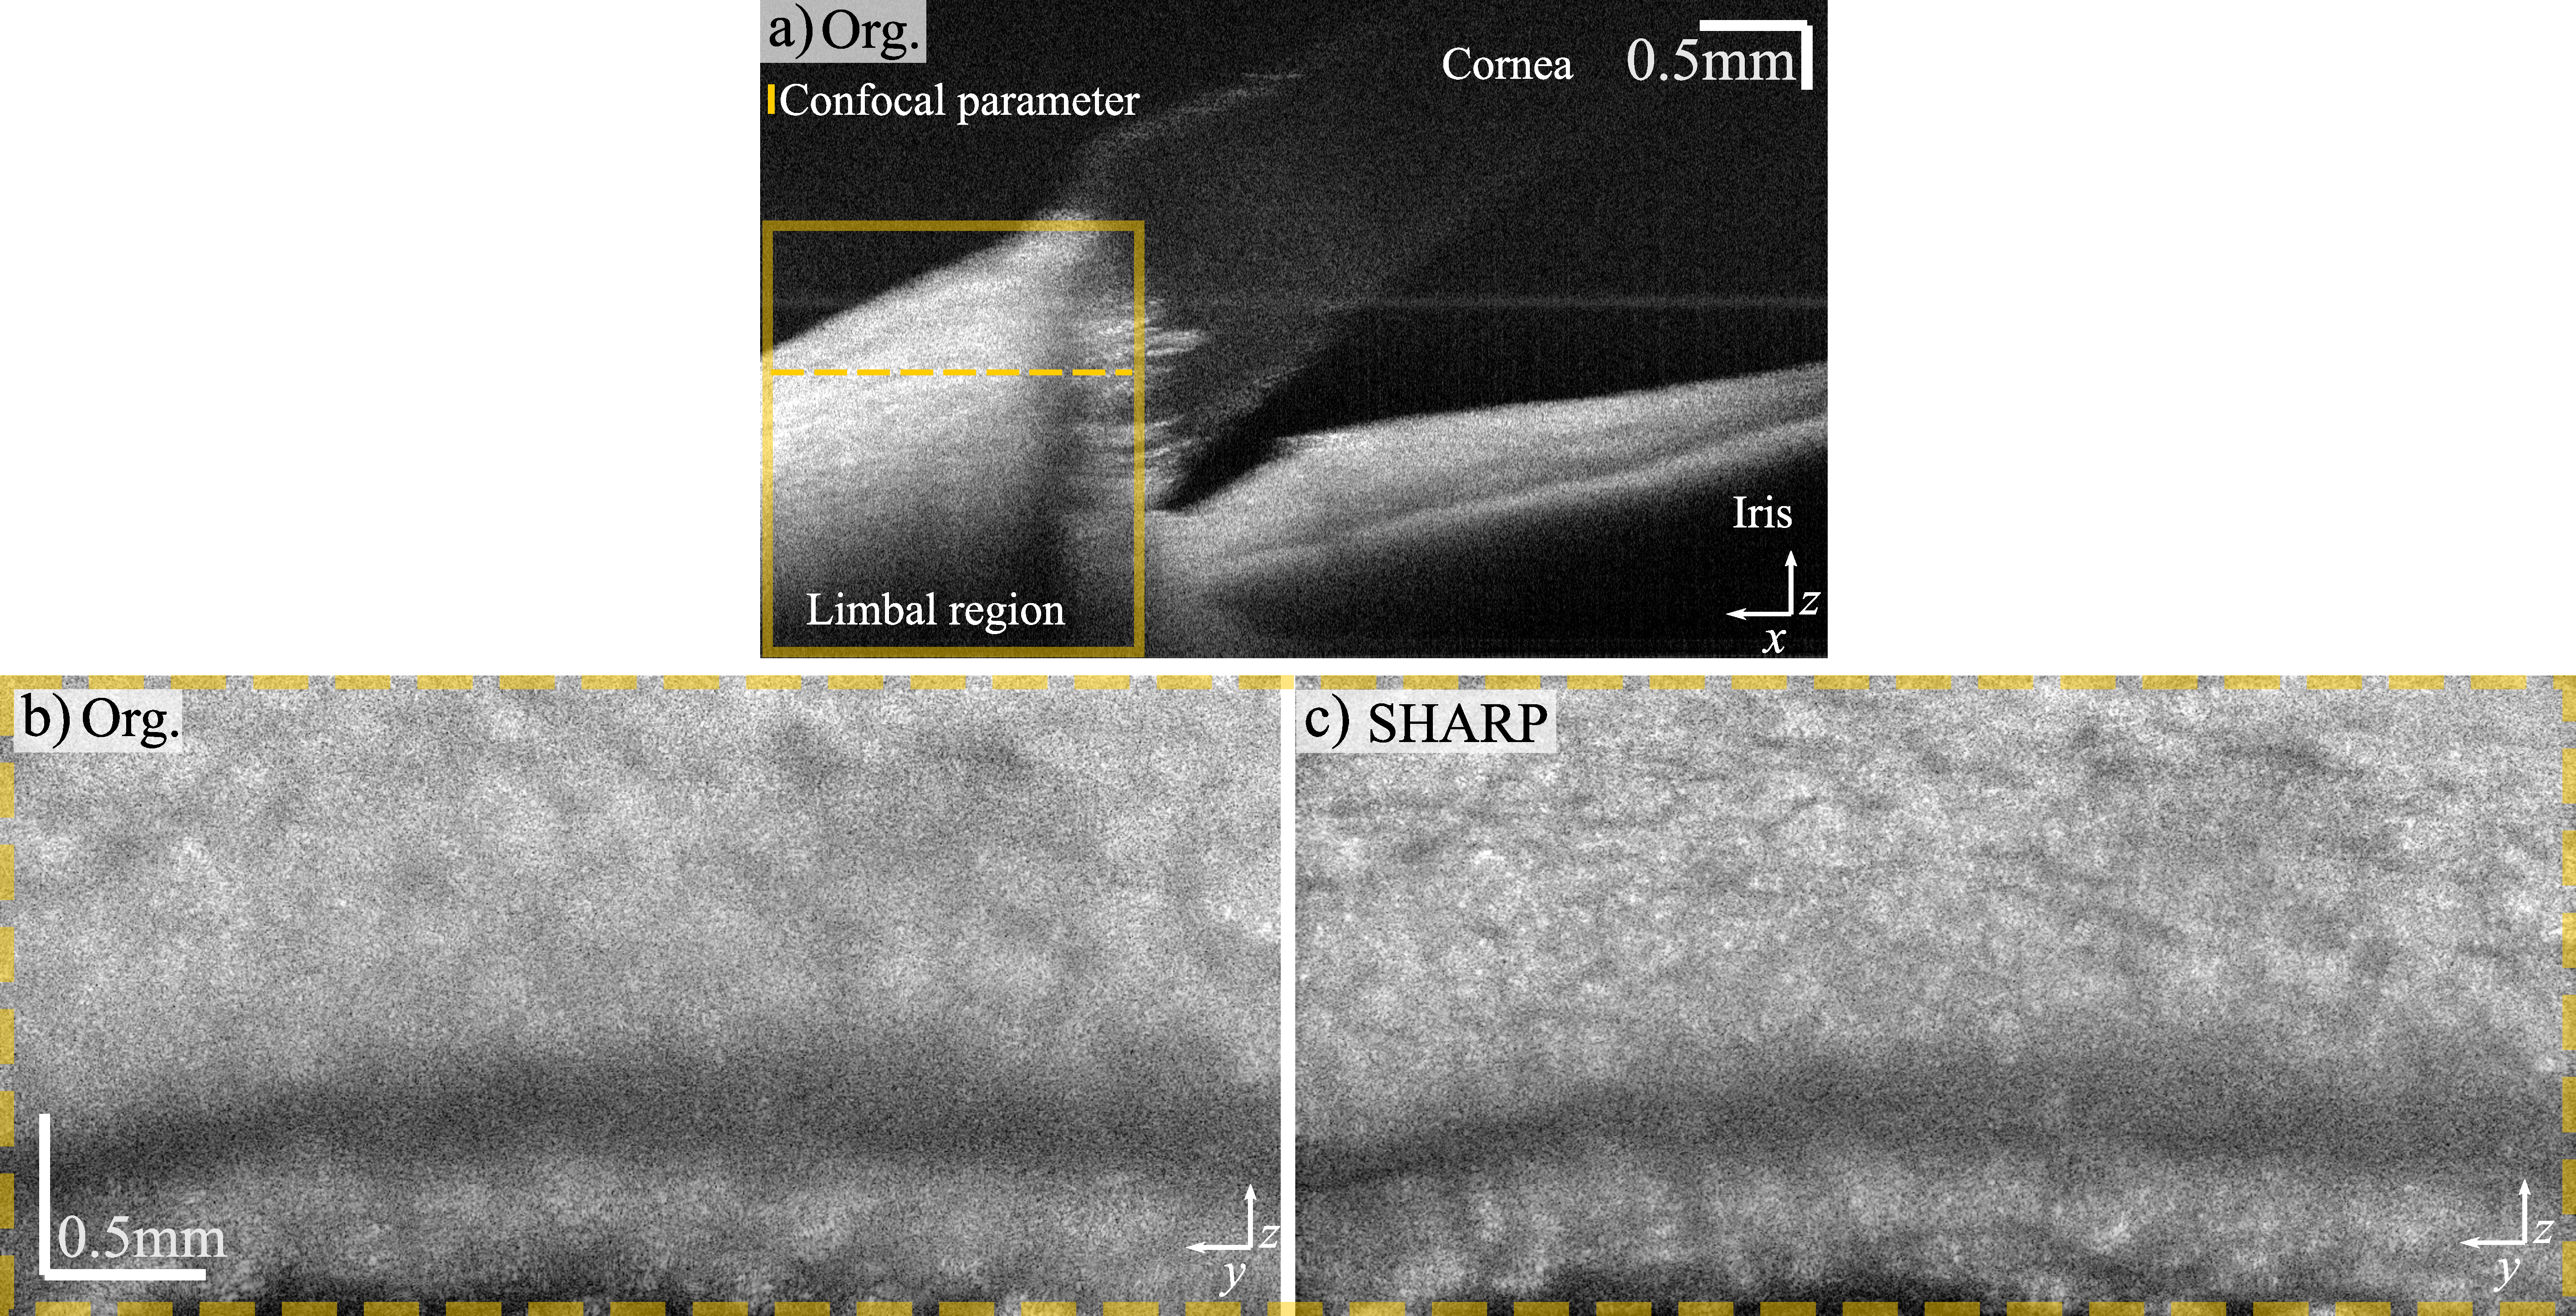
\includegraphics[width=\textwidth]{Figures/Results/PSOCT_Int.pdf}
	\caption[Application of SHARP in polarization-sensitive anterior segment imaging of an excised swine eye.]{Application of SHARP in polarization-sensitive anterior segment imaging of an excised swine eye. (a) B-scan around the limbal region. The limited depth of field is very apparent. The focus is near the center of the solid box. Dotted line indicates location of \textit{en face} views: (b) original (Org.) and (c) after SHARP.}
	\label{fig:PSOCT_int}
\end{figure}

Figure~\ref{fig:PSOCT} presents cross-sectional views after PS-OCT processing of the original and SHARP tomograms. Fig.~\ref{fig:PSOCT}(a) shows an intensity B-scan view with a yellow line marking the location of the cross-sectional views on Figs.~\ref{fig:PSOCT}(b)-(d), and a red line marking the location for the \textit{en face} views on Figs.~\ref{fig:PSOCT}(e)-(g); all insets show different tissue polarimetric parameters of the original data and the SHARP data side-to-side. The degree of polarization (DOP) is overlaid with the intensity in Figs.~\ref{fig:PSOCT}(b) and (e), local retardation is shown in Figs.~\ref{fig:PSOCT}(c) and (f) using a DOP threshold to display the intensity where DOP is $<0.65$, and the optic axis is overlaid with the local retardation in Figs.~\ref{fig:PSOCT}(d) and (g). Structures in the uncorrected images appear highly affected by defocus, spatial averaging and spectral binning. Polarimetric parameters calculated after SHARP do not exhibit any corruption in their information, furthermore successful refocusing is indicated by the clear improvement in spatial resolution in the polarimetric parameters, indicating that PS-OCT processing is indeed compatible with computational refocusing. Correcting for defocus reveals structures that appear blurred in the original tomograms, exhibiting better contrast and sharpness associated with the improvement of lateral resolution. This is noticeable in all polarimetric images, especially in the \textit{en face} views given that refocusing operates on both lateral axes. In particular, ridges-like structures can be visualized in the DOP images with SHARP, that may be associated with the Palisades of Vogt which are functionally important structures containing stem cells, associated with the regeneration of the corneal tissue after damage~\cite{Bizheva2017_Invivo}. 

\begin{figure}[htb!]
	\centering
	\includegraphics[width=\textwidth]{Figures/Results/PSOCT.pdf}
	\caption[Demonstration of computational refocusing in polarimetric parameters of the anterior segment of an excised swine eye.]{Demonstration of computational refocusing in polarimetric parameters of the anterior segment of an excised swine eye. (a) Intensity B-scan ROI around the solid box in Fig.~\ref{fig:PSOCT_int}. Cross-sectional views of tissue polarimetric parameters, showing original (Org.) and after SHARP side-to-side: (b), (e) DOP (isoluminant colormap) overlaid with intensity (luminance); (c), (f) local retardation for regions with DOP~$>0.65$ over the intensity; (d), (g) optic axis (cyclic isoluminant colormap) overlaid with local retardation (luminance). Axes of each cross-section are indicated in its corresponding panel.}
	\label{fig:PSOCT}
\end{figure}

There are two main limitations to the use of SHARP in PS-OCT. First, axial resolution of retardance and optic axis depend on the magnitude of spectral binning and the step size for local PS processing~\cite{Villiger2013_Spectral}. Thus, cross-sectional views [like Figs.~\ref{fig:PSOCT}(b)-(d)] show a less remarkable improvement than \textit{en face} views in which defocus is corrected in both axes [like Figs.~\ref{fig:PSOCT}(e)-(g)]. Axial resolution loss that occurs in spectral binning Stokes processing can be avoided using Mueller processing~\cite{Li2018_Robust} but in this case phase stability becomes relevant because input orthogonal polarization states have to be phase stable between them which currently is not achieved with SHARP. It could be possible to develop an strategy to leverage from the 1D phase stability like in SHARP but oriented to the tomograms from the two input polarization states to perform a full correction of the wavelength-dependent noise introduce by the system while maintaining the full axial resolution by using Mueller processing~\cite{Li2018_Robust}. Although this will limit spatial averaging to the axial and only one lateral dimensions, this could have attractive implications for the extraction of diattenuation information from tissue imaged with inter-A-line modulation PS-OCT systems, such as those used in intravascular OCT. Second, the improvement in lateral resolution after SHARP is partially neutralized by the spatial averaging required for PS-OCT processing. For this reason, advanced resolution-preserving despeckling is demanded in order to take full advantage of computational refocusing in PS-OCT. An extension of TNode to despeckle Stokes parameters is on current development, called polarization-sensitive-TNode (PS-TNode) and its combination with SHARP promises to be a powerful tool to improve and preserve resolution in PS-OCT imaging.